\documentclass[man,floatsintext]{apa6}
\usepackage{lmodern}
\usepackage{amssymb,amsmath}
\usepackage{ifxetex,ifluatex}
\usepackage{fixltx2e} % provides \textsubscript
\ifnum 0\ifxetex 1\fi\ifluatex 1\fi=0 % if pdftex
  \usepackage[T1]{fontenc}
  \usepackage[utf8]{inputenc}
\else % if luatex or xelatex
  \ifxetex
    \usepackage{mathspec}
  \else
    \usepackage{fontspec}
  \fi
  \defaultfontfeatures{Ligatures=TeX,Scale=MatchLowercase}
\fi
% use upquote if available, for straight quotes in verbatim environments
\IfFileExists{upquote.sty}{\usepackage{upquote}}{}
% use microtype if available
\IfFileExists{microtype.sty}{%
\usepackage{microtype}
\UseMicrotypeSet[protrusion]{basicmath} % disable protrusion for tt fonts
}{}
\usepackage{hyperref}
\hypersetup{unicode=true,
            pdftitle={Assessing sampling methods for generalization from RCTs: Modeling recruitment and participation},
            pdfauthor={Gleb Furman~\& James E. Pustejovsky},
            pdfkeywords={generalizability, sampling, MRT},
            pdfborder={0 0 0},
            breaklinks=true}
\urlstyle{same}  % don't use monospace font for urls
\usepackage{graphicx,grffile}
\makeatletter
\def\maxwidth{\ifdim\Gin@nat@width>\linewidth\linewidth\else\Gin@nat@width\fi}
\def\maxheight{\ifdim\Gin@nat@height>\textheight\textheight\else\Gin@nat@height\fi}
\makeatother
% Scale images if necessary, so that they will not overflow the page
% margins by default, and it is still possible to overwrite the defaults
% using explicit options in \includegraphics[width, height, ...]{}
\setkeys{Gin}{width=\maxwidth,height=\maxheight,keepaspectratio}
\IfFileExists{parskip.sty}{%
\usepackage{parskip}
}{% else
\setlength{\parindent}{0pt}
\setlength{\parskip}{6pt plus 2pt minus 1pt}
}
\setlength{\emergencystretch}{3em}  % prevent overfull lines
\providecommand{\tightlist}{%
  \setlength{\itemsep}{0pt}\setlength{\parskip}{0pt}}
\setcounter{secnumdepth}{0}
% Redefines (sub)paragraphs to behave more like sections
\ifx\paragraph\undefined\else
\let\oldparagraph\paragraph
\renewcommand{\paragraph}[1]{\oldparagraph{#1}\mbox{}}
\fi
\ifx\subparagraph\undefined\else
\let\oldsubparagraph\subparagraph
\renewcommand{\subparagraph}[1]{\oldsubparagraph{#1}\mbox{}}
\fi

%%% Use protect on footnotes to avoid problems with footnotes in titles
\let\rmarkdownfootnote\footnote%
\def\footnote{\protect\rmarkdownfootnote}


  \title{Assessing sampling methods for generalization from RCTs: Modeling recruitment and participation}
    \author{Gleb Furman\textsuperscript{1}~\& James E. Pustejovsky\textsuperscript{1}}
    \date{}
  
\shorttitle{Assessing sampling methods for generalization from RCTs}
\affiliation{
\vspace{0.5cm}
\textsuperscript{1} University of Texas at Austin}
\keywords{generalizability, sampling, MRT}
\usepackage{csquotes}
\usepackage{upgreek}
\captionsetup{font=singlespacing,justification=justified}

\usepackage{longtable}
\usepackage{lscape}
\usepackage{multirow}
\usepackage{tabularx}
\usepackage[flushleft]{threeparttable}
\usepackage{threeparttablex}

\newenvironment{lltable}{\begin{landscape}\begin{center}\begin{ThreePartTable}}{\end{ThreePartTable}\end{center}\end{landscape}}

\makeatletter
\newcommand\LastLTentrywidth{1em}
\newlength\longtablewidth
\setlength{\longtablewidth}{1in}
\newcommand{\getlongtablewidth}{\begingroup \ifcsname LT@\roman{LT@tables}\endcsname \global\longtablewidth=0pt \renewcommand{\LT@entry}[2]{\global\advance\longtablewidth by ##2\relax\gdef\LastLTentrywidth{##2}}\@nameuse{LT@\roman{LT@tables}} \fi \endgroup}
\usepackage{rotating}
\usepackage{float}
\geometry{twoside=false, top=1in, bottom=1in, left=1in, right=1.15in}
\usepackage[textwidth=1in, textsize=tiny]{todonotes}
\raggedbottom
\newcommand{\JEP}[1]{\todo[color=blue!20]{#1}}
\newcommand{\GF}[1]{\todo[color=orange]{#1}}

\authornote{

Correspondence concerning this article should be addressed to Gleb Furman, University of Texas at Austin, SZB 504, 1912 Speedway, Austin, Texas 78712. E-mail: \href{mailto:gleb.furman@utexas.edu}{\nolinkurl{gleb.furman@utexas.edu}}}

\abstract{
Educational research aimed at informing policy decisions must demonstrate that studies have been robustly designed to detect causal effects at the population level. Large scale multi-site randomized trials (MRT) often rely on vague convenience sampling methodology when recruiting districts and schools, resulting in relatively homogeneous samples that may differ greatly from the intended population of interest. Retrospective methods that quantify and statistically adjust for those differences are promising but may have difficulty overcomming substantial selection bias. Designing sampling methods that focus on generalizability may be a more effective (though costly) solution. However, limited methodological research has been performed to examine their effectiveness in the educational context. In this paper we develop a framework for conducting such research and propose methods to model recruitment and participation. Using this framework we then examine one promising method, stratified balanced sampling (SBS), in the context of recruiting a representative sample of schools for a large scale MRT. Using simulations based on real data, we compare SBS to stratified and unstratified versions of convenience sampling and probability sampling. Several models for generating school participation and emulating convenience sampling are proposed. Results indicate that SBS and stratified random sampling result in highly generalizable samples. These methods are extremely costly to implement, however, especially when the population average willingness to participate is low. Stratified convenience sampling is a potential compromise.


}

\begin{document}
\maketitle

\hypertarget{introduction}{%
\section{Introduction}\label{introduction}}

The multi-site randomized trial (MRT) has become a common design for evaluating the effectiveness of educational interventions. An MRT is a randomized control trial (RCT) that takes place across multiple distinct sites (e.g., school districts, medical clinics, or geographic areas), with random assignment taking place either at the site or unit level. In education research, implementing an MRT might entail recruiting multiple schools in each of several districts. Once a sample of schools is recruited, students, teachers, classes or whole schools are randomly assigned either to receive an intervention (treatment group) or to continue business as usual (control group).

Randomized treatment assignemnt supports a high level of internal validity, however using only a single site limits the external validity of the study. Though more costly, the advantage of using multiple sites is the ability to detect and account for cross-site variability. Ostensibly, this allows effect estimates to generalize to a larger population than estimates from a single-site design (Raudenbush \& Liu, 2000). However, the ambiguity in defining this larger popluation, as well as generalizability as a whole, has increasingly led MRTs to come under scrutiny.

In the context of intervention studies, generalizability describes how well the effect of an intervention would hold for units outside of the study. For instance, the sample average treatment effect (SATE) is a commonly reported point estimate for intervention effectiveness. Under certain circumstances, the SATE can a be reasonable estimate for the population average treatment effect (PATE) without any additional adjustments. In such cases, the intervention effectiveness detected in the study generalizes to the overall population of units from which the sample was taken. However, if response to intervention varies across units or sites, and the sample is compositionally different from the population of interest, then the SATE may no longer serve an unbiased estimate of the PATE.

The presence of treatment effect heterogeneity makes intervention effectiveness evaluations less informative to policy-makers who seek to make evidence-based decisions in populations that are outside of the study sample. Inadequate sampling strategies have been shown to be a major threat to generalizability of MRTs. Purposive or non-random samples may lead to substantially biased estimates of population-level effects (Olsen, Orr, Bell, \& Stuart, 2013; Shadish, Cook, \& Campbell, 2002). Several studies have found that schools and districts that participate in large scale randomized trials differ substantially from the national population (Fellers, 2017; Stuart, Bell, Ebnesajjad, Olsen, \& Orr, 2017). Beyond accurate effects estimates, generalizability can also be a question of equity. For instance, small under-served rural districts are underrepresented in RCTs sponsored by Institute of Education Sciences (Fellers, 2017; Stuart et al., 2017), and thus may be less likely to benefit from federally funded education research.

One way to achieve strong generalizability is to select sites from a well-defined population with known probabilities of selection. Assuming random assignment with full compliance and no attrition, this design enables unbiased estimation of the sample average treatment effect (SATE). Using the known sampling probabilities, the SATE can then be adjusted to estimate the population average treatment effect (PATE). Unfortunately, probability sampling is rarely used in large-scale impact evaluations (Olsen et al., 2013; Shadish et al., 2002). Instead, researchers often opt for convenience or purposive samples. These methods are much less expensive to implement, but are not usually designed to select a representative sample.

Provided several key assumptions hold, PATE can still be estimated from a non-random sample by using retrospective propensity score analyses (Kern, Stuart, Hill, \& Green, 2016; O'Muircheartaigh \& Hedges, 2014; Stuart, Cole, Bradshaw, \& Leaf, 2011; Tipton, 2013a). First, to justify claims about generalizability, the inference population must be well defined. Second, a set of covariates that predict treatment effect heterogeneity must be identified. Third, sampling is ignorable given a propensity score summarizing these covariates. Under these circumstances, SATE can be adjusted using inference population weights to estimate PATE.

A major shortcoming of such methods is under-coverage (Groves, 2004) which occurs when there are differences between the sample and inference population. This can be assessed using several techniques that identify how well a sample would generalize to a specific population (Stuart et al., 2011; Tipton, 2014). If under-coverage is great enough to prevent statistical adjustment of the SATE, then the inference population must be redefined. This can greatly diminish the relevance of study results and undermine the substantial investment into large-scale MRTs.

A series of recent papers instead advocate designing robust sampling methods that focus on generalizability at the recruitment stage (Tipton, 2013a, 2013b). These methods also require a well defined and enumerated population for which there is extant data, making them especially relevant in the educational context. One method in particular, Stratified Balanced Sampling (SBS), has received attention from intervention effectiveness researchers due to its accessibility. SBS involves using cluster analysis to split the population into smaller homogeneous strata to provide more manageable sub-populations for sampling. Sites within each stratum are then ranked according to how well they represent the stratum. Highly representative sites are then prioritized for recruitment. Researchers who are interested in using this to sample schools may even use a website (www.thegeneralizer.org) that guides them through this process using data from the Common Core of Data.

SBS can potentially reduce under-coverage, thereby improving the utility of retrospective methods for estimating PATE from non-random samples. Additionally, SBS requires meticulous documentation of decisions made during sampling which supports more transparency of recruitment methods. However, very little methodological work examining the method's effectiveness at selecting a generalizable sample has been reported. At least one research group has implemented SBS in the field and documented their experiences (Tipton \& Matlen, 2019). The authors reported success in selecting a highly generalizable sample, but substantial efforts were required to develop the sample frame, generate optimal strata, and coordinate with recruiters. This raises an important and pragmatic question: does the effectiveness of the method justify the additional resources necessary to implement it?

Additionally, though the recruiters reported that working within the strata did not burden their efforts, certain strata were more difficult to recruit from than others. Schools and districts with certain characteristics are unlikely to participate in large-scale MRTs (Fellers, 2017; Stuart et al., 2017; Tipton et al., 2016). If one or more strata are comprised of difficult schools, researchers might resort to convenience sampling within those strata, deviating from the balanced sampling design. This raises a further question of practicality: How effective is SBS if recruiters deviate from the initial protocol in favor of achieving the required sample size?

The goal of the current paper is two-fold. First, we propose several methods for modeling two major sources of sampling bias: recruitment and participation. Recruitment refers to how likely a population unit is to be approached by researchers. Specifically, we will examine SBS, simple random sampling and convenience sampling. The first two are fairly straightforward and can be described algorithmically. The latter, convenience sampling, can take on many forms in practice. We put forth a simple model of prioritizing sites that are likely to participate as a first step. To model the likelihood of a school participating, we will use extent demographic data and reported characteristics of schools that have been recruited to large-scale trials to generate a participation propensity score.

Second, using the models proposed in the first step, we report a simulation study comparing the performance of the sampling methods. The two criteria we will examine are as follows: (1) how generalizable is the sample attained by a given method and (2) how feasible was it to recruit a full sample using a given method. Feasibilty can be conceptualized in many ways. For the purposes of our study, we are mostly intersted in the difficulty which which a sample was selected, and how the likelihood of being sampled was distributed across the population. The former deals with costs to the researcher in terms of additional resources used to carry out a more comlex sampling design. The latter deals with costs to the schools in terms of the likelihood of being recruited.

As with many simulation studies, our scope will be limited to certain assumptions and simplifications. For instance, whether or not a school participates in a study is a complex and multifaceted decision, which we will simplify to a linear combination of demographic variables. Convenience sampling is also a complicated and poorly defined method for selecting a sample. Whether or not researchers approach a school may hinge on geographic proximity to the researcher, past relationships with administrators, features of the school district or surrounding city, or any combination of these and others predictors. Despite these two caveats, we feel that this study may still give us an insight into the relative performance of sampling methods.

The first section will provide an overview of SBS by demonstrating how it can applied to define strata and choose a generalizable sample. In the second section, we will propose a framework for studying sampling methods by proposing a model for participation behavior, and several models that prioritize schools for recruitment given a specified sampling method. In the third section, we describe how we implemented this framework in a simulation to study the relative performance of these methods. In the final two sections, we report our results and discuss limitations and directions for future research in this area.

\hypertarget{stratified-balanced-sampling}{%
\section{Stratified Balanced Sampling}\label{stratified-balanced-sampling}}

The goal of SBS is to recruit a study sample that is compositionally similar to a population of interest, such that treatment effects detected in the study can be generalized to that population. Covariates that potentially explain variation in treatment effects should be used to determine similarity. The multi-step process includes dividing the population into smaller homogeneous subgroups, prioritizing units representative of each subgroup for sampling, and refreshing the priority list after each round of recruitment. As such, SBS is an iterative process requiring collaboration between researchers and recruiters.

In this section we demonstrate SBS within the context of selecting schools for a large-scale MRT. This application will also serve as the basis for the subsequent simulation study. SBS is a flexible method that is adaptable to various data sets and, depending on study circumstances and design, may require different strategies or methods than presented here. For a more complete consideration of SBS, see Tipton (2013b).

SBS applies cluster analysis as a dimension reduction technique to drive bias-robust balanced sampling based on a large set of covariates. The ultimate goal is to select a sample that is representative of a population with respect to a set of covariates related to treatment heterogeneity and site participation. This process requires the availability of a rich data set of observed covariates for each site in the population. We therefore begin by discussing the data which will serve as the sampling frame and the covariates we have selected.

Following recommendations proposed by Tipton (2013b), we then implement k-means clustering to divide the population into heterogeneous strata comprised of homogeneous sites. K-means clustering assigns sites to strata such that similarity within each stratum is maximized. This step requires us to specify the number of strata that need to be generated. Here we rely on empirical criteria as well as subjective appraisals of what is feasible to implement.

After determining the strata, we then use a second distance metric to rank sites in order of how representative each site is of its stratum. These ranks are later used to drive \enquote{balanced sampling} by prioritizing sites for recruitment. In practice, these rankings should encourage the selection of sites from subsets of the population which may otherwise not have been included given typical sampling strategies.

Finally, we discuss the advantages and limitations of SBS given our implementation, and the potential difficulties of using this to sample schools in the greater context of educational research.

\hypertarget{sample-frame}{%
\subsection{Sample Frame}\label{sample-frame}}

We first identify a population of schools from which we want to select a representative sample. Six states served as the geographic boundaries for this sample frame: California, Oregon, Pennsylvania, South Carolina, Texas, and Wyoming. These six states were selected because they provided ready access to additional school and district level achievement data, which can be used to expand the current research.

The cluster analysis depends on a complete enumeration of all population units and access to covariates that moderate treatment effects. Since we are only interested in selecting a representative sample, we instead identified covariates that predict school participation in RCTs. The goal is for our final sample to include schools not normally found in large-scale evaluations of interventions. To this end, selection of covariates was driven by prior research on district and school participation behavior in RCTs (Stuart et al., 2017; Tipton et al., 2016a; Fellers, 2017). These studies found that districts and schools with higher proportions of students who are English language learners (ELL), economically disadvantaged (ED), non-White, and living in urban settings are more likely to participate, as are larger districts and schools.

It is important to note that some of these characteristics might also make it more likely that researchers would recruit these districts and schools in the first place. That is to say, school characteristics may drive selection bias by both impacting the types of schools that agree to participate, as well as by the types of schools that researchers recruit. For instance, the over-representation of larger schools in RCTs can mean that schools with more students are: (a) more likely to agree to participate, (b) more likely to be recruited by researchers, or (c) some combination of both (a) and (b). Therefore, the participation behavior outlined here is likely not representative of all schools in the US, rather only schools that are likely to be recruited by current practices.

\begin{figure}
\centering
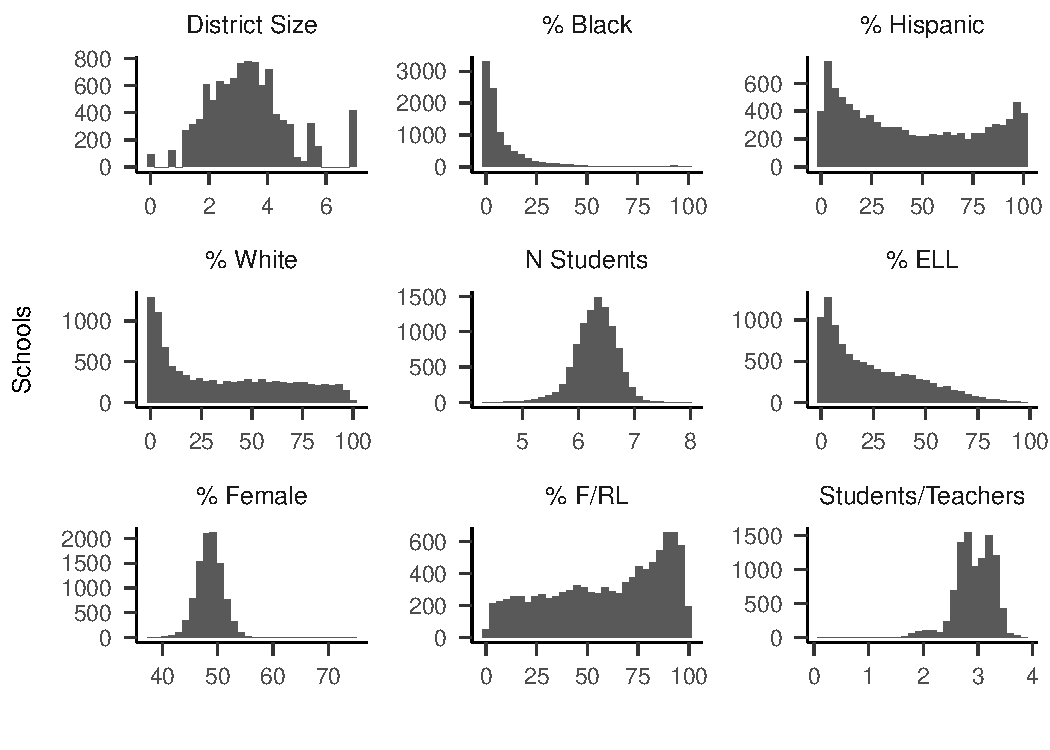
\includegraphics{GenSamp-Paper_files/figure-latex/plot-dist1-1.pdf}
\caption{\label{fig:plot-dist1}Distributions of continuous covariates. Three covariates were transformed to logs: District Size, N Students, and Student/Teachers}
\end{figure}

We sourced the characteristics of the sample frame from the Common Core of Data (CCD; \url{https://nces.ed.gov/ccd/index.asp}). The CCD is a comprehensive database housing annually collected census data of all public schools and districts. We calculated log-transformations of school size (number of students), district size (number of schools) and the student to teacher ratio. This was done to allow proportional comparisons at the extremes of the distributions (Hennig \& Liao, 2013). For instance, the difference between two schools with 4000 and 3000 students was weighed as much as the difference between two schools with 400 and 300 students when generating clusters. Figure \ref{fig:plot-dist1} displays the distribution of the continuous variables used. Two categorical covariates were used as well: urbanicity (urban, suburban, or town/rural) and a binary indicator of school wide title 1 eligibility. In all, the sample frame consists of 6 states, 2,016 districts and 9,792 schools.

\hypertarget{stratification}{%
\subsection{Stratification}\label{stratification}}

Sample stratification is commonly used in survey sampling and large-scale experiments to reduce the variance of an estimate. Often this is done with one or two covariates that lend themselves to categorization (Lohr 1999). Since our purpose is to reduce bias in the estimate by controlling for potential moderators, we will require a far larger number of covaraites of varying complexity. Traditional stratification at this scale would result in too many strata to handle and an overly complicated recruitment process..

Instead, a dimension reduction tool is used to condense the population into smaller set of homogeneous strata. Per Tipton (2013b)'s original recommendation, we implement k-means clustering to partition the population into a pre-determined number of strata. This requires selecting a distance metric, specifying the number of strata, and generating the strata. All analyses were performed in R (R Core Team, 2018).

\hypertarget{cluster-analysis}{%
\subsubsection{Cluster Analysis}\label{cluster-analysis}}

We performed the cluster analysis using the \emph{cluster} package (Maechler et al., 2017). First, the \emph{daisy} function is used to compute an \(n\) by \(n\) pairwise distance matrix across all observations. This function requires two parameters: (1) the data matrix, and (2) the distance metric. The data matrix includes the full set of school level covariates used to compare schools for clustering. The distance metric summarizes the difference between a pair of sites on a set of covariates in order to maximize the similarity of all sites within a cluster. As such, the appropriate metric varies depending on the type of data in the matrix.

In educational research, as is the case here, data are likely to contain both continuous and categorical variables. For mixed data such as this, it is appropriate to use the general similarity measure (Gower, 1971; Tipton, 2013b). This measure relies on different calculations of distance depending on the type of covariates. Let \(X_{hi}\) and \(X_{hi'}\) be the observed value of covariate \(h = {1, ..., P}\) for sites \(i\) and \(i'\) respectively, where \(i \ne i'\). Let \(d_{ii'h}\) be the distance between observed values of covariate \(X_{h}\) for site \(i\) and site \(i'\). For categorical or dummy coded variables, \(d_{ii'h} = 1\) if \(X_{hi} = X_{hi'}\) and \(d_{ii'h} = 0\) otherwise. For continuous covariates, we use the following formula:
\begin{align}
d_{ii'h} = 1 - \frac{|X_{hi} - X_{hi'}|}{R_h}
\end{align}
where \(|\cdot|\) indicates absolute value, and \(R_h\) is the range of observations for covariate \(X_h\). This equation restricts the range of \(d_{ii'h}\) to \([0,1]\). Finally, we calculate the general similarity between each site pair by taking the weighted average of the distances between all covariates. Let \(d^{g}_{ii'}\) be the general similarity between site \(i\) and site \(i'\).
\begin{align}
d^{g}_{ii'} = \frac{\sum^p_{h = 1}w_{ii'h}d_{ii'h}}{\sum^p_{h = 1}w_{ii'h}}
\end{align}
where \(w_{ii'h} = 0\) if \(X_h\) is missing for either site and \(w_{ii'h} = 1\) otherwise. Setting the distance metric to \enquote{gower} in the \emph{daisy} function performs these calculations.

\hypertarget{number-of-strata}{%
\subsubsection{Number of Strata}\label{number-of-strata}}

Next we used the \emph{kmeans} function to generate clusters, which employs an optimization algorithm to classify sites into \(k\) clusters by minimizing the total within cluster variance. For each \(k\), it is recommended to run \emph{kmeans} at least 10 times, and select the clustering that results in the smallest total within-cluster sum of squares. This function also requires two parameters: (1) the distance matrix from the previous step, and (2) the number of clusters to generate (\(k\)).

Selecting an appropriate value for \(k\) is one of the most difficult problems in cluster analysis (Steinley, 2006). Tipton (2013b) states that both empirical and practical criteria should be used in selecting \(k\). Hennig and Liao (2013) also argue that the method of selecting \(k\) should depend on the context of the clustering, framing the issue as one of obtaining an appropriate subject-matter-dependent definition rather than a statistical estimation.

Proportional allocation dictates that each stratum should contribute a number of units to the full sample that is proportional to the size of the strata. Having unequal sized strata means that recruiters will need to focus more on larger strata. Generating a larger set of strata would result in greater homogeneity within each stratum, however it may also be more difficult to manage for recruiters. For instance, if refusal and non-response rates are fairly high, having fewer sites spread across more strata may make it difficult to adequately recruit from all strata. Resource constraints (e.g.~time, funding, recruiters) may also be a factor in the number of strata selected.

With these considerations in mind, we examined three criteria: (1) a generalized form of the Calinski-Harabasz index (Cali\a'nski \& Harabasz, 1974) proposed by Hennig and Liao (2013), (2) the proportion of between-cluster variance as recommended by Tipton (2013b), and (3) the practicality of sampling from fewer clusters. Our strategy was to perform the analysis several times for each value of \(k\) and compare all performance criteria for each set of strata generated (Figure \ref{fig:fig-k-plots}).

We first calculated the Calinski-Harabasz (CH) index using the \emph{cluster.stats} function from the \emph{fpc} (Hennig ???) package. Figure \ref{fig:fig-k-plots}a displays the CH index for each \(k\) clusters generated. In this case, generating 2 clusters maximizes the CH-index. Another potential solution is at 5 clusters where there is also a local maxima.

\begin{figure}[tbp]
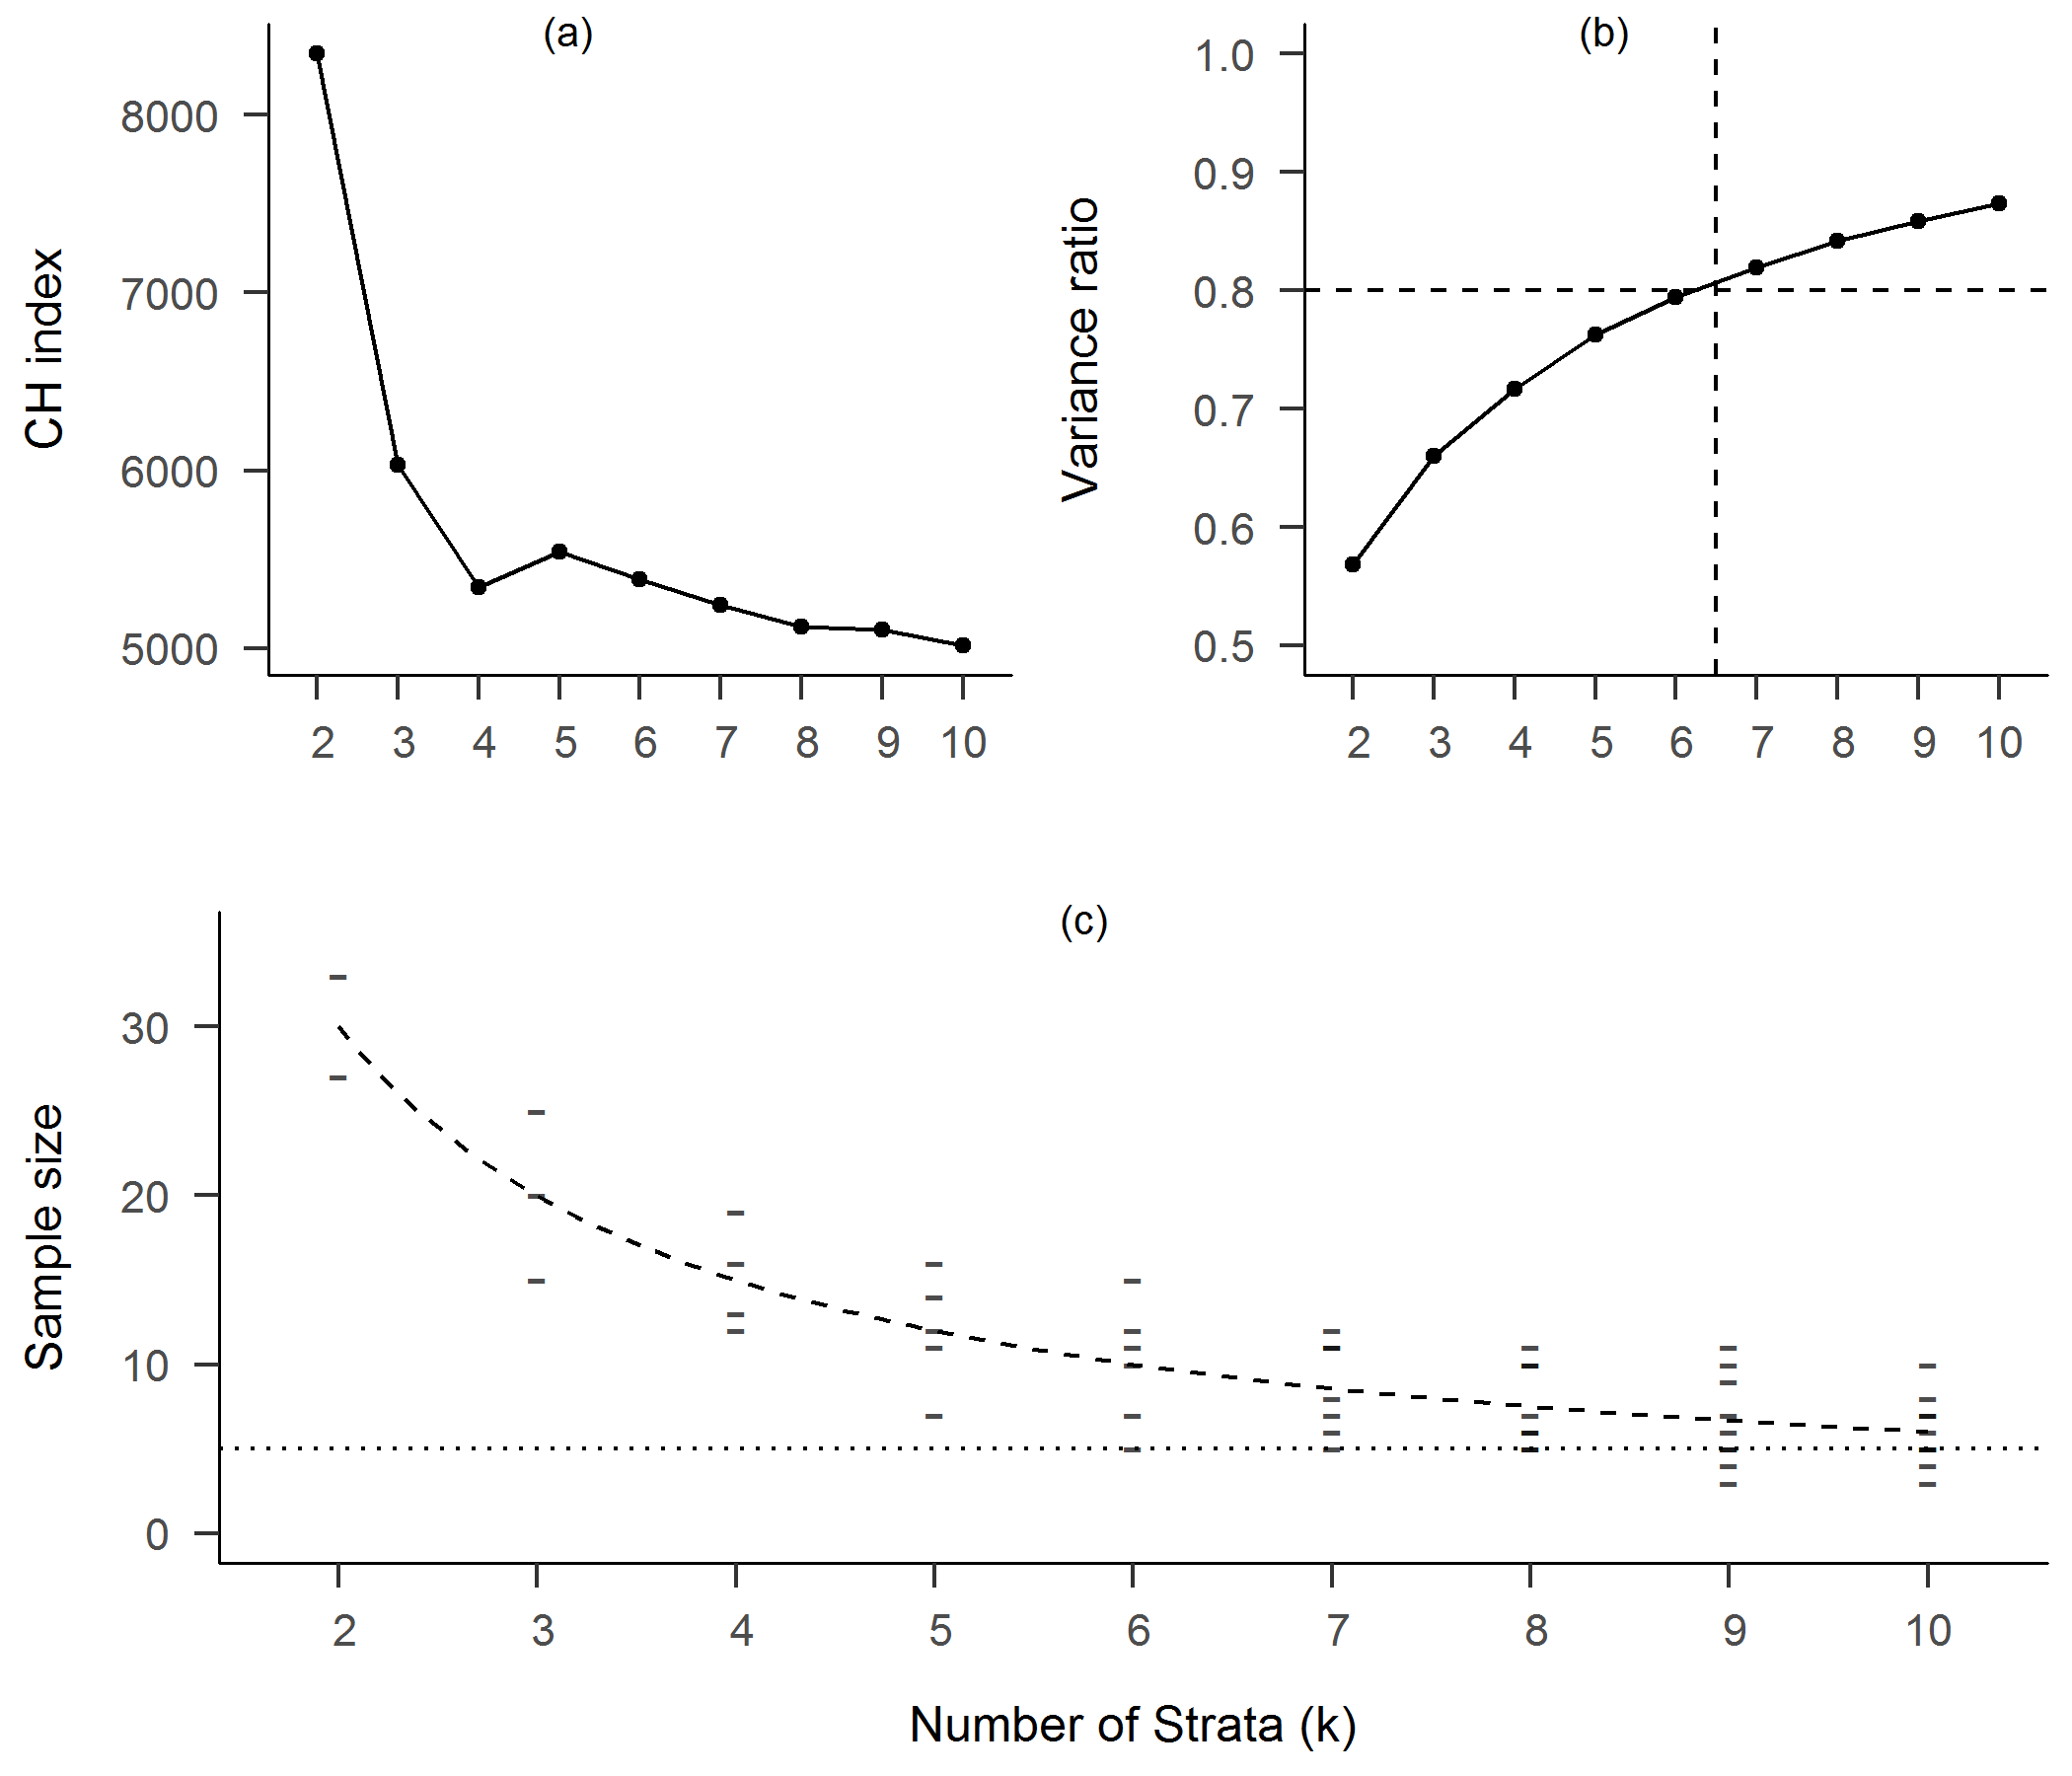
\includegraphics[width=1\linewidth]{GenSamp-Paper_files/figure-latex/fig-k-plots-1} \caption{Plots used to determine value for $k$. (a) Calinski-Harabasz index; peaks indicate better fit. (b) Ratio of between cluster sum of squares to total cluster sum of squares; horizontal line indicates cutoff of .8, vertical line indicates minimum number of clusters needed to achieve cutoff. (c) Sampling requirements for each cluster given proportional allocation; horizontal line indicates a cluster sample size requirement of 5 schools.}\label{fig:fig-k-plots}
\end{figure}

The proportion of between-cluster variance was calculated manually. Let \(k\) be the number of strata generated where \(k = 1, 2, ..., q\) for some maximum allowable number of \(q\) strata. For each set of \(k\) strata, we compute the between and within cluster variability for each covariate. Summing these values across all covariates gives us the total variability within strata (\(\sigma_{wk}^2\)) and the total variability between strata (\(\sigma_{wk}^2\)). We then calculate the proportion of variability that is between strata for each set of \(k\) strata as:

\begin{align} \label{eq:pk}
p_k = \sigma_{bk}^2/(\sigma_{wk}^2 + \sigma_{bk}^2)
\end{align}
As \(p_k\) approaches 1, most of the variation is between strata, indicating homogeneity within strata. This increases the possibility of selecting a more balanced sample.

Figure \ref{fig:fig-k-plots}b plots \(p_k\) against \(k\). The \(k\) for which the rate of change \(p_k\) slows is considered favorable. Tipton (2013b) also recommends selecting the number of clusters such that at least 80\% of the variability is between clusters, indicated by the figure as a dashed line. In light of this criterion, it seems that at least 7 clusters should be generated. However, we also see that after a sharp initial increase, the slope of the graph begins to level out. This indicates that as we increase the number of clusters, the benefit of doing so decreases, while the difficulty of sampling from each cluster increases. In practice, the difficulty of sampling may not be worth the small increases in homogeneity within clusters obtained when using at least 5 clusters.

Figure \ref{fig:fig-k-plots}c plots the sample size that needs to be selected from each cluster to fulfill the proportional allocation requirement. The dashed line indicates the ideal allocation if all clusters were of equal size. We see that the variability in cluster sizes decreases as more clusters are generated. A sensible cutoff may be determined by looking at the size of the smallest cluster. At \(k > 6\) it seems that the smallest clusters would require less than 5 sites being sampled, which may be very difficult in a practical setting. We determined that this would be the most likely criteria to be considered in the field, and ultimately decided to generate 5 clusters for this analysis.

\hypertarget{balanced-sampling}{%
\subsection{Balanced Sampling}\label{balanced-sampling}}

The goal of balanced sampling is to recruit in such a way that the expected value of covariate \(X_h\) across sites in stratum \(j\) is equal to the expected value of covariate \(X_h\) across all sites sampled from stratum \(j\):
\begin{align}
E(X_{hi}|Z_i = 1, j) = E(X_h|j)
\end{align}
where \(Z_i = 1\) if site \(i\) is recruited into the sample and \(Z_i = 0\) otherwise. Following Tipton (2013b), we implemented balanced sampling by prioritizing the recruitment of sites based on their similarity to the \enquote{average} site in each stratum. First we identified the number of sites to be sampled from each stratum using proportional sample allocation. Each stratum contains \(N_j\) sites where \(N_1 + N_2 ... + N_k = N\). From each stratum \(j\), we calculated the number of sites to be sampled, \(n_j\), such that \(n_j = [(N_j/N)n]\), where {[}.{]} indicates the value rounded to the nearest integer.

Next we ranked each site within a stratum using a distance measure, with sites closer to the \enquote{center} of the strata ranked higher. We calculated the weighted Euclidean distance to the mean of each covariate:
\begin{align} \label{eq:euclid}
d_{ij} = \sqrt{\sum^p_{h=1}w_h(X_{hij} - \mu_{hj})^2}
\end{align}
where \(w_h\) is the weight assigned to covariate \(X_h\), \(\mu_{hj}\) is the population mean of covariate \(h\) in stratum \(j\), and \(X_{hij}\) is the value of covariate \(h\) for site \(i\) in stratum \(j\). As with generating the strata, different weights can be used such that distances depend more heavily on covariates thought to be more related to treatment effect heterogeneity. To weigh covariates equally, we set the weight weight of a covariate to the inverse of its population variance as \(w_h = 1/\sigma^2_h\). We then used the ranked list to prioritize sites for recruitment, beginning with the highest ranked sites. If a site was unavailable or refused to participate, a recruitment attempt was made with the next highest ranked site until \(n_j\) sites agreed to participate.

\hypertarget{advantages-and-limitations}{%
\subsection{Advantages and Limitations}\label{advantages-and-limitations}}

Though there are very few demonstrations of SBS in the literature, several studies outline the method's theoretical benefits (Tipton, 2013b; Tipton et al., 2016). First, SBS requires that researchers document the recruitment process, carefully consider the inference population, and justify targeting specific sites. This supports transparency and enables a more careful critique of the sampling design and study inferences. Second, careful documentation also supports follow-up analysis on participation behavior such as systematic differences across non-responders. Finally, SBS easily integrates with post-hoc statistical adjustment techniques. Even if balance is only partially improved at the sampling stage, coverage errors will still be reduced and less of the inference population will need to be discarded during analysis.

There are, of course, several limitations as well. SBS depends on the existence of a rich set of observed covariates related to treatment heterogeneity and sample selection for each site in the population. Most readily available extant data primarily consist of demographics and may not contain information on covariates that are more proximally related to variation in treatment effect. This can result in omitted variable bias during the cluster analysis phase (Tipton, 2013b). Additionally, SBS requires more resources to implement than a simple convenience sample. Recruiting ranked sites from multiple strata requires a coordinated effort between recruiters (Tipton, Hallberg, Hedges, \& Chan, 2017). This means that recruiters cannot work independently and must rely on a partnership with researchers implementing this method.

At least one study documents the complete implementation of SBS in a large-scale multi-site educational intervention study (Tipton \& Matlen, 2019). The authors reported that a substantial amount of time had to be dedicated to developing the sampling frame and generating optimal strata. This was compounded by the unavailability of data necessary for identifying the sampling frame. For instance, some schools were ineligible for the study due to their curriculum not aligning with the intervention. Such information may only become apparent once a school is selected and contacted directly, adding a frustrating level of trial and error to the recruitment process.

The recruitment effort also required a considerable amount of coordination between the researchers and the recruiters. However, the researchers were able to elicit buy-in from the recruiters, who in follow-up interviews reported that the recruitment plan and its benefits were easy to understand. Furthermore, the recruiters felt that working with strata constraints did not increase the difficulty of recruitment, though they did find that some strata were easier to recruit from than others.

\hypertarget{methods-and-models}{%
\section{Methods and Models}\label{methods-and-models}}

In this section we develop the framework for designing a simulation study of recruitment in educational research. First, we operationalize the ultimate goal of selecting a generalizable sample. Next, we consider how to introduce selection bias using a combination of models for participation behavior and recruitment behavior. Modeling selection bias accurately is critical to the validity of this research. However, this depends on some knowledge of recruiter and participant behavior which is fairly limited in the current literature. The models we propose are by no means comprehensive, instead they serve as a first step into this line of research.

\hypertarget{framework-for-generalizability}{%
\subsection{Framework for Generalizability}\label{framework-for-generalizability}}

Following the framework developed by Tipton (2013b), we begin with a data set enumerating a population of \(N\) sites (schools), indexed as \(i = 1 ... N\). Each site also has a vector of observed characteristics \(X_i\) of length \(p\). The covariates are a mixture of continuous, binary, and categorical data. The goal is to select a sample of \(n\) sites such that there is balance along \(X_i\) between the sample and the population, indicating that the population is compositionally represented by the sample. We measure balance using the standardized mean difference (\(SMD\)) between the sample and population for a given covariate. \(SMD\) is calculated as

\begin{align} \label{eq:SMD}
SMD = \frac{\bar{X}-\mu}{\sigma}
\end{align}
where \(\bar{X}\) is a vector of covariate means in the sample, \(\mu\) is the vector of covariate means in the population, and \(\sigma\) is the vector of covariate standard deviations in the population. \(SMD\) values closer to zero indicate greater balance between the sample and the population.

\hypertarget{modeling-selection-bias}{%
\subsection{Modeling Selection Bias}\label{modeling-selection-bias}}

Selection bias stems from two sources: (1) site participation behavior (self-selection) and (2) researcher sampling behavior (recruitment bias). To model the former we propose a simple participation propensity score. Let \(\pi^P_i\) represent the participation propensity score, or the probability that site \(i\) agrees to participate in an RCT if approached for recruitment. Using a simple logistic transformation we model \(\pi^P_i\) as follows:
\begin{align} 
\label{eq:RGM}
log\bigg(\frac{\pi^P_i}{1 - \pi^P_i}\bigg) = \beta_0 + \boldsymbol{x_i \beta}
\end{align}
where \(\boldsymbol{x_i}\) is an \(1\) by \(p\) matrix of covariates that predict sample selection for each site, and \(\boldsymbol{\beta}\) is a vector of coefficients associated with those covariates. Participation for site \(i\) will be determined by sampling from a Bernoulli distribution with probability equal to \(\pi^P_i\).

Modeling recruitment bias is less straightforward. While self-selection is present as long as sites have the ability to choose whether or not to participate, recruitment bias depends largely on whatever strategy is used for selecting sites in the first place. It can be avoided all together by using probability sampling techniques, where the probability that a site will be invited to participate is known and can be accounted for in the outcome analysis. However, this is not often feasible in the case of large-scale MRTs. Subsets of schools are likely to be overlooked if samples are too small, or when participation rates are too low. Further, random sampling from a broad population (such as an entire country) is likely to produce samples that are geographically dispersed, creating logistic difficulties for data collection and treatment implementation. As a result, researchers often eschew probability sampling in favor of convenience sampling (Gerber \& Green, 2012; Shadish et al., 2002).

Since researchers rarely operationalize and report their process for selecting a convenience sample, the question of what drives recruitment bias, and how to model it, is left largely open-ended. As a first step, we will entertain the strong assumption that the purpose of convenience sampling is to minimize effort. If we further assume that recruiters have some prior knowledge of how likely schools are to participate if approached, then we can model this selection mechanism as recruiters prioritizing schools with a higher propensity to participate. We refer to this as the \enquote{low hanging fruit} approach to convenience sampling.

\hypertarget{sampling-methods}{%
\subsection{Sampling Methods}\label{sampling-methods}}

In this section we propose formal models for several sampling procedures. These procedures, which will be incorporated in the simulation study, are not meant to be comprehesnive. However, by formalizing them in this fashion we hope to make the procedures transparent, reproducible, and modifiable to easily fit other circumstances which may be of interest for study.

We will be comparing 5 sampling methods in the simulation study: stratified and unstratified random sampling, stratified and unstratified convenience sampling, and stratified balanced sampling (SBS). We model the sample selection process in two stages. In the first stage, we generate indicators of \emph{potential participation}---that is, whether a school would participate in the trial \emph{if approached for recruitment}. Let \(N\) be the total number of schools in the population, and let schools be indexed by \(j = 1, ..., N\). We define \(E_j\) as a binary indicator that school \(j\) will agree to participate if contacted by recruiters, where \(E_j = 1\) if the school agrees, and \(E_j = 0\) if the school refuses. Each school is checked for approval by sampling from a Bernoulli distribution with probability equal to \(\pi^P_j\) for each school \(j\)
\begin{equation}
\label{eq:Ej}
E_j \sim B(\pi^P_j)
\end{equation}
In this manner, \(\pi^P_j\) is constant as it represents a school characteristic, and \(E_j\) can vary across iterations.

We model the sampling process as observing the potential participation indicator for schools in a ranked list, where the order in which schools are contacted is determined by a score \(S = S_1,...,S_N\). Let \(Z_j(S)\) be an indicator whether school \(i\) is sampled based on the score \(S\).
For the unstratified sampling methods, we determined \(Z_1(S),...,Z_N(S)\) by sorting schools according to \(S\) and selecting the first 60 schools where \(E_j = 1\).
Specifically,
\begin{equation}
\label{eq:Zj}
Z_j(S) = I\left[60 \geq \sum_{k=1}^N E_k I\left(S_k \leq S_j\right)\right]
\end{equation}
where \(I(C)\) denotes the indicator function, equal to 1 if \(C\) is true and otherwise equal to 0. Based on the sample selection indicators, we calculate the number of schools contacted as
\begin{equation}
\label{eq:R}
R(S) = \sum_{j=1}^N I(S_j \leq S_{max}),
\end{equation}
where \(S_{max} = \max \{S_1 Z_1, S_2 Z_2, ..., S_N Z_N\}\).

For the stratified sampling methods, the above process is applied within each stratum. We determine target sample sizes for each stratum based on proportional sample allocation described previously. Letting \(N_k\) denote the total number of schools in stratum \(k\), we set a target sample size of \(n_k = [60 \times N_k / N]\) for stratum \(k\), where \([x]\) is the integer nearest to \(x\).

\hypertarget{random-sampling}{%
\subsubsection{Random Sampling}\label{random-sampling}}

As previously mentioned, unstratified random sampling (URS) is typically highly impractical in the context of educational MRTs. However, URS is nonetheless interesting as a theoretically simple ideal against which to compare other sampling methods. We can simulate URS sampling by ranking each school according to a random number from a uniform distribution, so that their order of recruitment is determined by the score \(S_j \sim U(0, 1)\).

In practice, methods such as cluster sampling, stratified sampling, or a combination of both would likely offer advantages over unstratified random sampling. We therefore also simulate a stratified random sample (SRS), with strata determined by the results of the cluster analysis and using a proportional allocation.

\hypertarget{convenience-sampling}{%
\subsubsection{Convenience Sampling}\label{convenience-sampling}}

We also simulate two convenience sampling methods: unstratified (UCS) and stratified convenience sampling (SCS). Here, we assume that recruiters have some knowledge of each schools' probability of participating, if approached, and that they prioritize higher probability schools in order to minimize effort. To operationalize unstratified convenience sampling, we assume that schools are approached for recruitment one at a time, with their order determined by sampling without replacement, and with probability proportional to participation propensity scores \(\pi^P_1,...,\pi^P_N\).
Once a school is selected and assigned a rank, the next school is selected with a probability proportional to the weights of the remaining schools. Once all ranks are assigned, schools are again approached until 60 schools agreed to be in the sample. We implemented stratified convenience sampling using the same process, but with ranks determined independently within each stratum, and using a proportional allocation across strata.

\hypertarget{balanced-sampling-1}{%
\subsubsection{Balanced Sampling}\label{balanced-sampling-1}}

SBS is unique in that rankings are directly related to school characteristics and do not change across iterations. Scores within strata are based on equation \eqref{eq:euclid} (i.e., \(S_j = d_{jk}\)), where schools closer to the \enquote{center} of the stratum are more representative of it and are therefore a higher priority. Though extremely unlikely, it is possible that several schools could be equidistant from the center of the stratum; in such cases, schools are ordered randomly. Because Tipton (2013b) proposed balanced sampling in connection with stratification based on a cluster analysis, we only consider the stratified version, SBS.

\hypertarget{simulation-study}{%
\section{Simulation Study}\label{simulation-study}}

In this section we describe the simulation study developed to assess the generalizability of the samples selected by SBS relative to several other sampling methods, and the feasibility with which the sampling methods can be employed. A simulation study is the most convenient method for comparing multiple sampling techniques in a controlled environment. The external validity of this study largely rests on our ability to accurately model the participation propensity score. By relying on previous work and real data to inform our model, we hope to maximize how well our results represent reality.

\hypertarget{data-generation}{%
\subsection{Data Generation}\label{data-generation}}

\hypertarget{strata-assignments}{%
\subsubsection{Strata Assignments}\label{strata-assignments}}

In the Stratification section, we detailed how the cluster analysis was performed and resulted in schools being assigned to one of five strata. Strata are tied diectly to school characteristics, and are independant of any of the simulation study's conditions. Strata assignments are therefore constant accross iterations and conditions.

\hypertarget{participation-propensity-score}{%
\subsubsection{Participation Propensity Score}\label{participation-propensity-score}}

We modeled the participation propensity score (equation \eqref{eq:RGM}) using observed covariate values from extant school data. The set of covariates, \(X_i\), consisted of the same variables used in the cluster analysis described in Sample Frame section above. The corresponding coefficients, \(B\), were based on work by Fellers (2017) who compared 571 elementary schools that participated in IES funded studies to the full population of U.S. elementary schools. The authors reported absolute SMD between the schools that participated and the population. We standardized \(X_i\) and used reported SMDs as coefficients in equation \eqref{eq:RGM} to generated \(\pi^P_i\) values. The covariates along with the coefficient values are reported in Table \ref{tab:tab-RGM-Pars}. We generate different levels of population participation rates by manipulating the intercept values. Since these rates are unknown, we selected parameters for 9 levels of participation rates. As such, participation propensity scores were constant for each school only within each participation rate condition.

\begin{table}[tbp]
\begin{center}
\begin{threeparttable}
\caption{\label{tab:tab-RGM-Pars}Odds ratio coefficients for Response Generating Model}
\begin{tabular}{ll}
\toprule
Variables & \multicolumn{1}{c}{log\_odds}\\
\midrule
District Size & 0.52\\
\% Black & 0.29\\
\% Hispanic & 0.40\\
\% White & -0.54\\
N Students & 0.37\\
\% ELL & 0.41\\
\% Female & -0.02\\
\% F/RL & 0.08\\
Students/Teachers & -0.10\\
Suburban & 0.01\\
Schoolwide Title I & 0.02\\
Town/Rural & -0.40\\
Urban & 0.43\\
\bottomrule
\end{tabular}
\end{threeparttable}
\end{center}
\end{table}



\hypertarget{simulation-procedures}{%
\subsection{Simulation procedures}\label{simulation-procedures}}

We designed the simulation to examine the performance of 5 sampling methods across 9 levels of population participation. The population of schools and their assigned strata were constant across all conditions and iterations. The participation propensity score was constant across all sampling methods and iterations within each level of population participation. Within each iteration, all schools were checked for approval (equation (8)) which then remained constant accross each sampling method. That is, if a school happened to be approached by three sampling methods within an iteration, the school would provide the same response to all three methods (agree or refuse to participate). The order in which schools were approached varied by method and across iterations. The one exception is the balanced sampling method, where the order in which schools are approached is constant since it is tied to strata assignemnt and school characteristics.

In total, 45,000 samples were generated by running 1000 iterations for each of 9 population participation levels, and using 5 sampling methods in each iteration. Each iteration proceded as follows. First, we generated school responses (\(E_j\)) for all schools. Next, we generated 5 sets of rankings, one for each sampling method, for all schools. We checked each school in order of rank for recruitment until a sample of 60 schools was selected by each method. For each sample within an iteration, we tracked which schools aggreed to participate, which schools refused to participate, and how many schools refused to participate. We also calculated the B-index and the SMD between each sample and the population. If the sampling method was a stratified version, B-indicies and SMDs were calculated within each stratum as well.

\hypertarget{analysis}{%
\subsection{Analysis}\label{analysis}}

\hypertarget{generalizability}{%
\subsubsection{Generalizability}\label{generalizability}}

There are several methods to quantify how generalizable a sample is to a target population. One common method is to compare the sample to the population on a range of covariates by examining SMDs as shown in equation \eqref{eq:SMD}. This method is limited as it only provides us with a measure of how close the sample means are to the population means. To have true generalizability, sample variance must also be representative of the population variance. Therefore, in addition to SMDs we also estimated the generalizability index (\(B\); Tipton, 2014).

The generalizability index is bounded between 0 and 1, with 0 indicating no overlap between the sample and the population, and 1 indicating the sample is representative of the population.

\begin{align}
B = \int_{\pi_{min}-3h_{max}}^{\pi_{max}-3h_{max}}\sqrt{\hat{f}_s(z)\hat{f}_p(z)}dz
\end{align}

where \(\hat{f}_s(z)\) is a Gaussian kernel density estimate of sample distribution of propensity scores using bandwidth \(h_s\), and \(\hat{f}_p(z)\) is a Gaussian kernel density estimate of population distribution of p-scores using bandwidth \(h_p\). We calculate the bandwidth \(h\) for the population or sample as follows:

\begin{align}
h(\pi_i,...,\pi_n) = \sigma_{\pi}(\frac{4}{3n})^{1/5}
\end{align}

where \(\sigma_{\pi}\) is the variance of the propensity scores. \todo[color=orange]{Do these equations look right? Should (11) be $\pi_{max}+3h_{max}$?}

\hypertarget{feasibility}{%
\subsubsection{Feasibility}\label{feasibility}}

To assess feasibility, the total number of schools approached to achieve a full sample was tracked. The average number of refusals each sample method resulted in prior to selecting the full sample was calculated across replications. Recruiters expend a lot of resources contacting districts and schools, scheduling meetings and traveling between interested locations. A project with limited resources may not be able to afford to go through a large list of potentially uninterested sites. This measure allows us to compare the difficulty with which a full sample is recruited using each method.

\hypertarget{sampling-inequality}{%
\subsubsection{Sampling Inequality}\label{sampling-inequality}}

To assess sampling inequality, we tracked the frequency with which schools were recruited by each sampling method across iterations and conditions. We then summarized this data by calculating the Gini coefficient for each method. This was done in R using the \emph{Gini} function from the \emph{ineq} package (Zeileis 2014). The Gini coefficient is typically used in economics to assess the degree of income inequality by showing the disproportionate distribution of wealth across levels of incomes. Similarly it could be used in the context of sampling by identifying how often under-represented schools are recruited to participate in studies. The Gini index ranges from 0 to 1, with 0 indicating perfect equality, and 1 indicating perfect inequality.

\hypertarget{results}{%
\section{Results}\label{results}}

\hypertarget{generalizability-1}{%
\subsection{Generalizability}\label{generalizability-1}}

\hypertarget{b-index}{%
\subsubsection{B-Index}\label{b-index}}

Figure \ref{fig:fig-avg-Bindex} displays the average \(B\)-index for each method across participation rates. Acceptable values of \(B\) for generalizability vary depending on the size of the sample, the size of the population, and the number of covariates (Tipton, 2014). Given our design, a value of \(B = .95\) would be needed to expect full generalizability, with lower values requiring additional statistical adjustment. At population participation rates below 50\%, only SBS consistently selected highly generalizable samples. This indicates that SBS is successful at sampling schools that are unlikely to participate and therefore tend to be underrepresented by the other sampling methods---particularly when overall participation propensities are low. Stratified random sampling consistently outperformed simple random sampling across all participation rates, though only slightly.

\begin{figure}
\centering
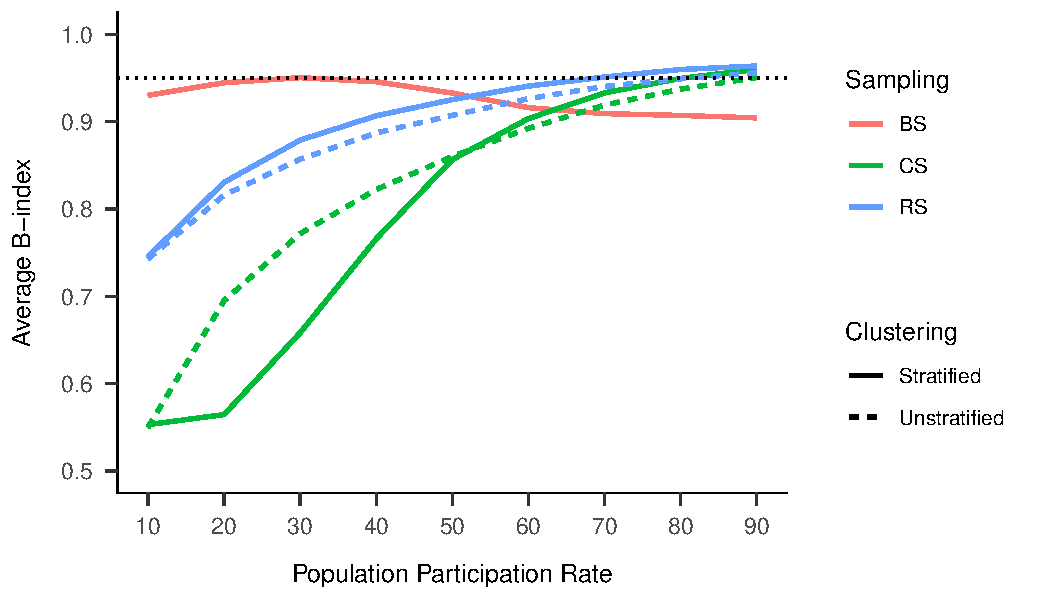
\includegraphics{GenSamp-Paper_files/figure-latex/fig-avg-Bindex-1.pdf}
\caption{\label{fig:fig-avg-Bindex}Average \(B\)-index for varying participation rates, by sampling method. Horizontal dotted line represented index of .95 indicating a high level of generalizability.}
\end{figure}

We also found several trends that were unexpected. At 50\% and beyond, SBS performance slowly degrades, while other methods maintain a steady increase. We expected a constant positive relationship between the population participation rate and the performance of all methods. Furthermore, at low response rates unstratified convenience sampling seemed to perform better than stratified convenience sampling. This seems counter-intuitive, as survey literature suggests that stratified samples are more representative. Because the B-index is an overall measure of generalizabilty across many covariates, it is difficult to untangle why these methods preformed as they did. We next examined the performance of the sampling methods on each individual covariate.

\hypertarget{standardized-mean-differences}{%
\subsubsection{Standardized Mean Differences}\label{standardized-mean-differences}}

We began this analysis by plotting mean SMDs for each covariate across all sampling methods against the population participation rate. Sampling methods were considered to perform well if they resulted in an average SMD value below .25 across iterations. The relative performance of the sampling methods were used to group covariates into four patterns of performance. The first group of covariates is displayed in figure \ref{fig:fig-SMD-by-Var-good1}, where all stratified methods resulted in good balance along these covariates, while unstratified methods resulted in poor balance, especially in lower population participation rates. Notably, SBS always performed better or as well as the other stratified methods.

\begin{figure}
\centering
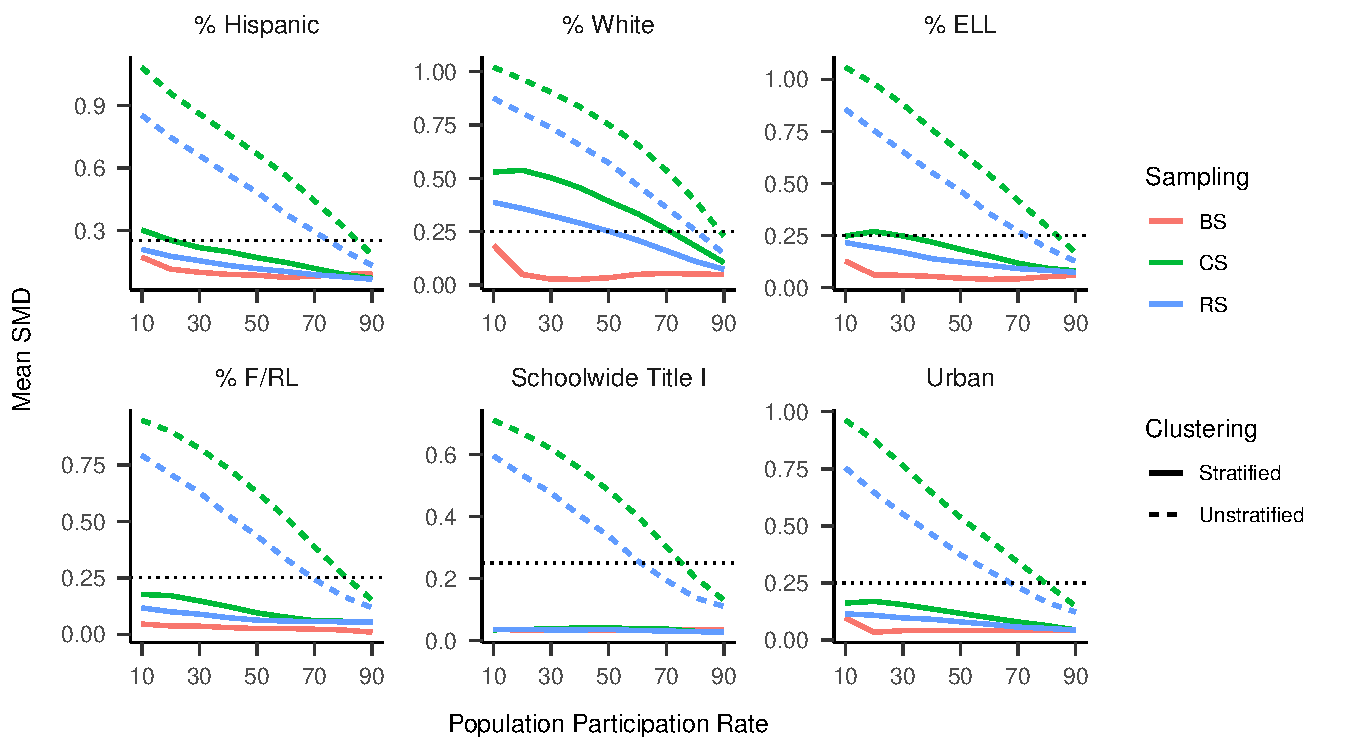
\includegraphics{GenSamp-Paper_files/figure-latex/fig-SMD-by-Var-good1-1.pdf}
\caption{\label{fig:fig-SMD-by-Var-good1}Group 1, good balance for stratified methods, poor balance for unstratified methods at low participation rates. Dotted horizontal line indicates a .25 cutoff.}
\end{figure}

The second group of covariates is displayed in figure \ref{fig:fig-SMD-by-Var-good2}. Here, the stratified sampling methods consistently outperform their unstratified counterparts. However, in some conditions, SCS performed worse than URS, or even SBS. Also, SBS was outperformed by SCS and SRS in certain conditions. The third group of covariates is displayed in figure \ref{fig:fig-SMD-by-Var-neutral}. Here, all sampling methods resulted in good balance across all population participation rates. SBS seemed to perform slightly better than all other methods, while differences between the other methods seems negligible. Finally, the fourth group of covaraites is displayed in figure \ref{fig:fig-SMD-by-Var-bad}. For these covariates, SBS performed consistently well across population participation rates. However, URS and UCS performed better than their stratified counterparts.

\begin{figure}
\centering
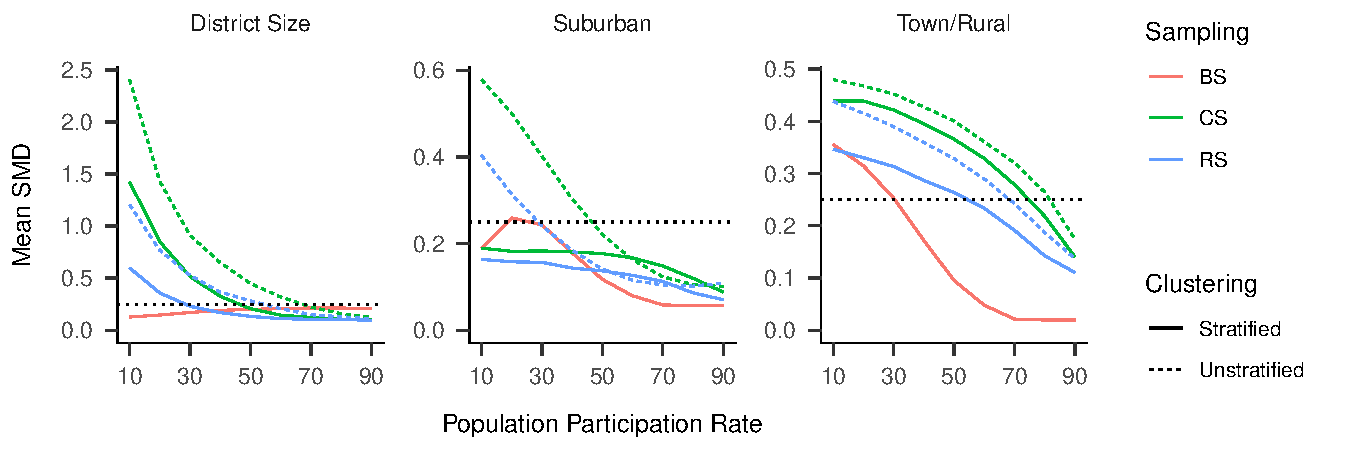
\includegraphics{GenSamp-Paper_files/figure-latex/fig-SMD-by-Var-good2-1.pdf}
\caption{\label{fig:fig-SMD-by-Var-good2}Group 2: good balance for stratified versions of methods, inconsistent performance by SBS and ScS. Dotted horizontal line indicates a .25 cutoff.}
\end{figure}

\begin{figure}
\centering
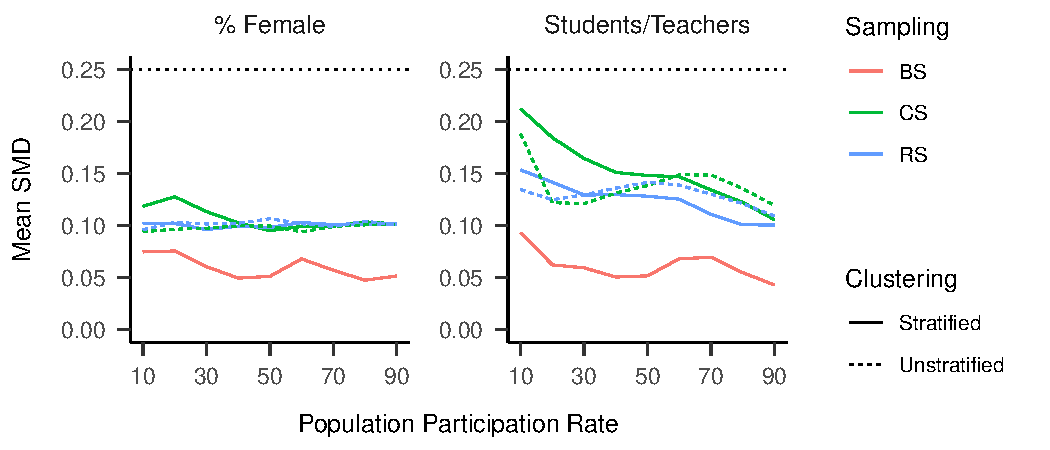
\includegraphics{GenSamp-Paper_files/figure-latex/fig-SMD-by-Var-neutral-1.pdf}
\caption{\label{fig:fig-SMD-by-Var-neutral}Group 3: all methods performed well, with SBS performing slightly better. Dotted horizontal line indicates a .25 cutoff.}
\end{figure}

\begin{figure}
\centering
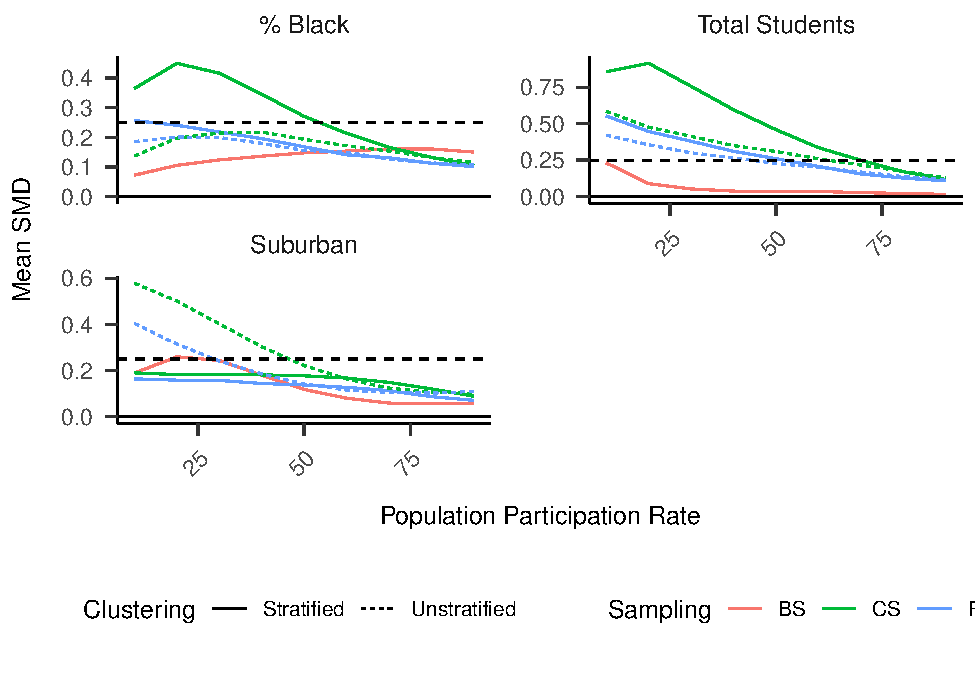
\includegraphics{GenSamp-Paper_files/figure-latex/fig-SMD-by-Var-bad-1.pdf}
\caption{\label{fig:fig-SMD-by-Var-bad}Group 4 - poor relative performance for stratified convenience sampling and stratified random sampling. Dotted horizontal line indicates a .25 cutoff.}
\end{figure}

One potential explanation for why including stratification in a sampling design may result in poorer balance is that the strata are poorly specified. This may occur if the strata do not explain any variance in a covariate that is related to participation. To examine this we calculated the ICC for each covariate (i.e., the proportion of variance in the covariate that was between strata) and compared it to the log-odds coefficients associated with that covariate in the participation propensity model. We then plotted these values in figure \ref{fig:fig-ICCvsCoef}.

We noted several interesting relationships when examining the groups of covariate previously described,. Group 3, where all sampling methods performed well, consisted of covaraites that were fairly unrelated to participation, and which played almost no role in generating strata. Group 4, where stratification seemed to reduce the performance of sampling methods, consisted of covaraites that were predictive of participation, but were also overlooked by the strata generation process.

\begin{figure}
\centering
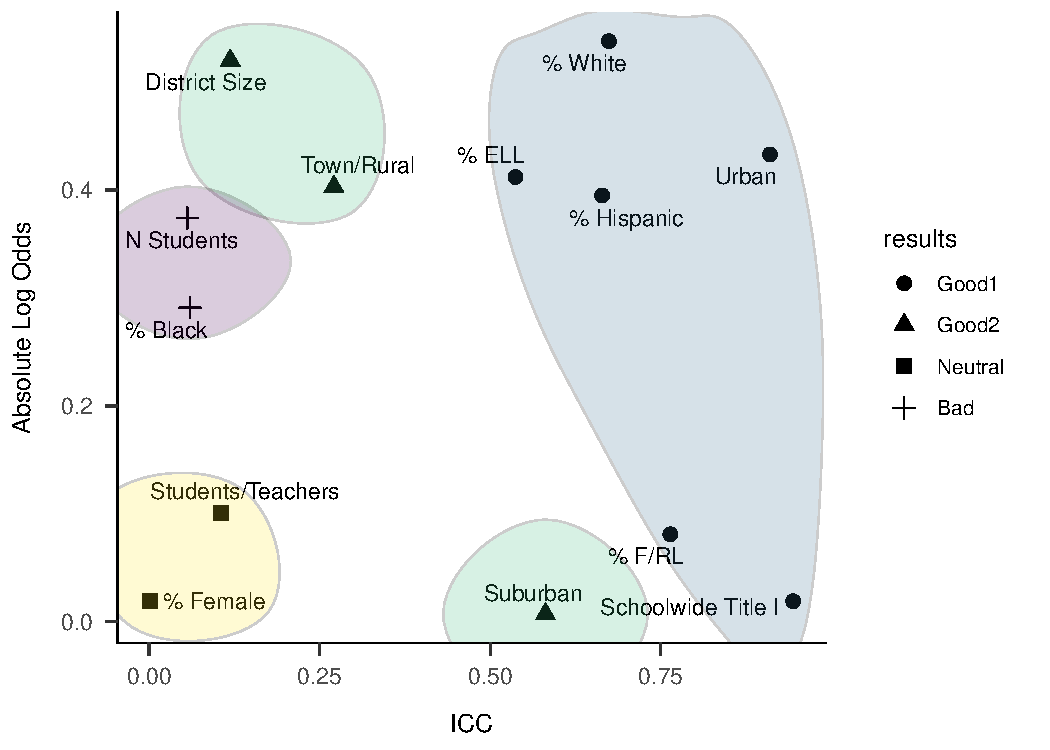
\includegraphics{GenSamp-Paper_files/figure-latex/fig-ICCvsCoef-1.pdf}
\caption{\label{fig:fig-ICCvsCoef}ICC Values vs absolute log odds. Shaded areas illustrate potential patterns in generalizability measured by SMDs.}
\end{figure}

\hypertarget{feasibility-1}{%
\subsection{Feasibility}\label{feasibility-1}}

\hypertarget{recruitment-attempts}{%
\subsubsection{Recruitment Attempts}\label{recruitment-attempts}}

Figure \ref{fig:fig-responses}a reports the total number of units that needed to be contacted to recruit a full sample of 60 schools across population participation rates for all sampling methods. Figure \ref{fig:fig-responses}b reports the percent of schools that agreed to participate across population participation rates for all sampling methods. Differences between sampling methods along these two measures were substantial at lower participation rates. As participation rates increased, the differences decreased exponentially and became negligible. It is important to note that the magnitudes of these results are quite extreme. This is likely due to some misspecification on the part of the simulation either in the response generating model parameters or the population participation rates. Rather than looking at the raw values, a more meaningful interpretation would be to compare the performance of the models relative to each other. Overall, UCS required the least \enquote{effort} to recruit a full sample, followed by URS and SCS, SRS, and finally SBS.

\begin{figure}
\centering
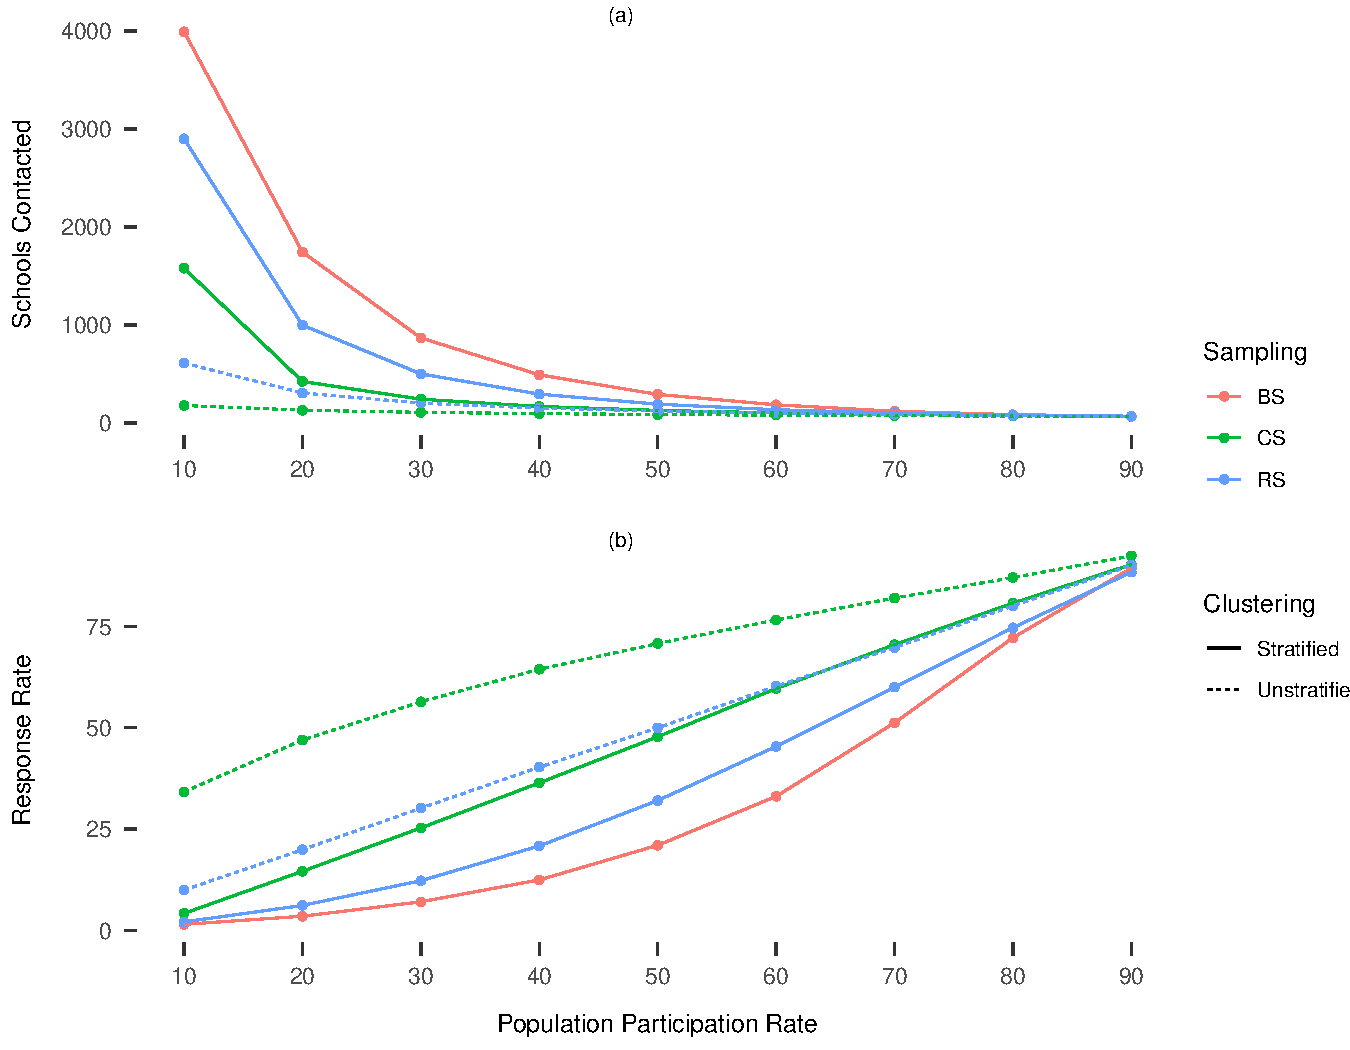
\includegraphics{GenSamp-Paper_files/figure-latex/fig-responses-1.pdf}
\caption{\label{fig:fig-responses}Sample recruitment statistics and response rates. Plot (a) shows the total number of units contacted to achieve a full sample of 60 schools. Plot (b) shows the percent of schools that agreed to participate when recruited.}
\end{figure}

\hypertarget{inequality-of-selected-samples}{%
\subsubsection{Inequality of selected samples}\label{inequality-of-selected-samples}}

We calculated the Gini coefficient for each sampling method to examine the equality of sampling probabilities across methods. Figure \ref{fig:fig-gini} displays these for each sampling method across population participation rates. A coefficient of 1 indicates substantial sampling inequality. In the context of the simulation, a high Gini coefficient indicates that across iterations, only a small subset of the population was ever actually recruited.
Several trends emerged in this analysis. As population participation rates increased, inequality increased when using SBS, but decreased when using any other method. These four other methods also performed consistently relative to one another, with SRS resulting in the least amount of sampling inequality, followed by URS, SCS and UCS. As population rates increased, differences between stratified and unstratified versions of sampling methods seemed to decrease. This finding suggests that stratifying the population results in a larger potential sampling pool when the overall population response rate is low.

\begin{figure}
\centering
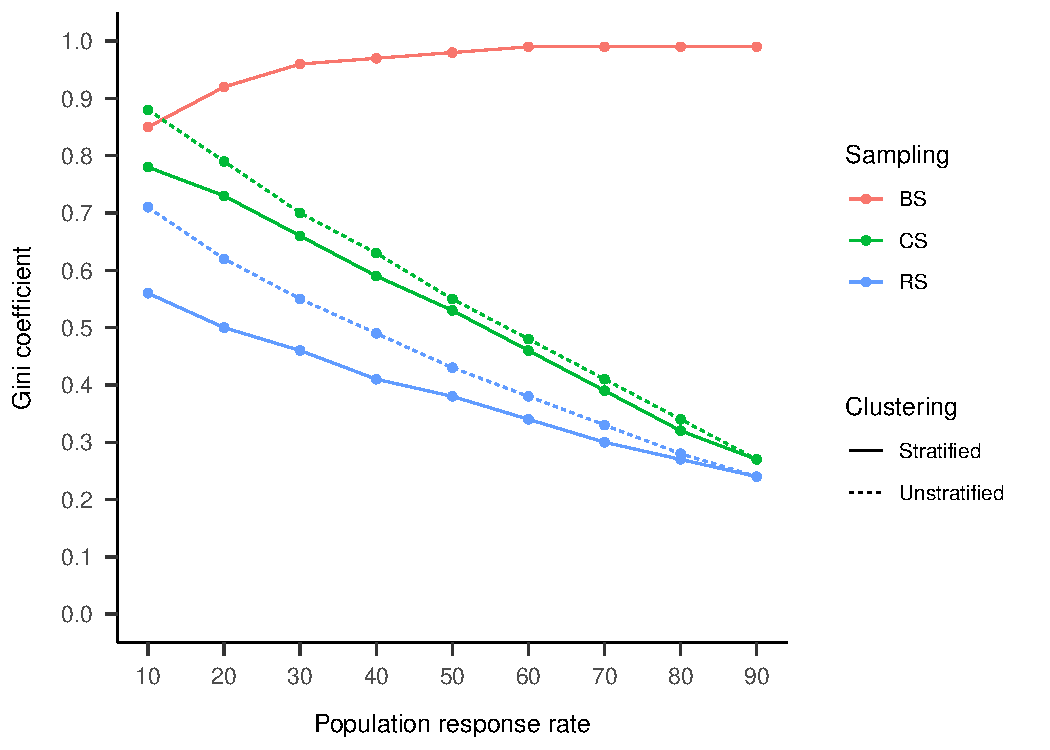
\includegraphics{GenSamp-Paper_files/figure-latex/fig-gini-1.pdf}
\caption{\label{fig:fig-gini}Gini coefficient across participation response rates for each sampling method. A coefficient of 1 indicates major inequality in sampling probability.}
\end{figure}

\hypertarget{summary-of-trends}{%
\subsection{Summary of Trends}\label{summary-of-trends}}

In terms of selecting a generalizable sample, SBS resulted in a considerable improvement compared to UCS. However, given the difficulty with which those samples are recruited, SBS is unlikely to be fully implemented in the ideal form. Instead, SCS may be a reasonable compromise. Our findings indicate that convenience and probability sampling methods are often improved by first stratifying the population. In certain cases, convenience sampling within strata (SCS) is comparable to simple random sampling (URS) both in terms of generalizability and feasibility.

An important observation which has not yet been addressed in the literature relates the specification of the clustering method to the response model. For instance, in Figure \ref{fig:fig-SMD-by-Var-bad} we see that all methods of sampling result in balance on percentage of Black students, except for stratified convenience sampling. This is likely a result of the covariate having a strong relationship with participation, but not being weighed enough in the cluster analysis used in determining the strata. Figure \ref{fig:fig-ICCvsCoef} displays the calculated intraclass correlation coefficient (ICC) for each covariate along the strata, and the coefficient for each covariate in the response generating model. For covariates where one value (ICC or coefficient) is high, while the other is low, stratified sampling techniques resulted in poorer balance.

\hypertarget{discussion}{%
\section{Discussion}\label{discussion}}

The main goal of this study was to develop a framework for exploring the performance of sampling methods within the educational context. We put forth several models for algorithmically representing how researchers may select convenience sample of schools. Using prior work we also attempted to model how schools may decide whether or not to participate in a study if approached by recruiters. The methods we proposed for modeling these behaviors can, in principle, be extended to more complex and realistic specifications and adapted to other population frames.

A secondary goal was to use this framework in a demonstration of several sampling methods and their relative performance in terms of generalizability and feasibility. From this work we have drawn several conclusions. Stratified balanced sampling as proposed by Tipton (2013b) has the potential to greatly increase the generalizability of samples selected for MRTs. However, this method is not without limitations. Within our simulation, strict adherence came at a great cost in terms of sheer number of schools that needed to be contacted. Thus, implementing this method in practice may require allocating many more study resources to sample recruitment.

We found that ignoring the response model when specifying covariate weights during the cluster analysis stage may attenuate the generalizability of the resulting sample. Covariates that were not prioritized when generating the strata wound up being poorly represented in the final samples if they strongly predicted participation. Ignoring these relationships has the potential to undermine the investment of resources into SBS. Finally, while the balanced sampling approach does result in greater generalizability, it also appears to limit the actual pool of potential participants. Particularly in larger population response rates, the same subset of schools were likely to be recruited across iterations.

One potential compromise between current practice and SBS is to generate strata, but then implement convenience sampling within strata. As demonstrated in the simulations, stratified convenience sampling often resulted in better balance on individual covariates than simple random sampling. This may also elicit greater buy in from recruiters by placing less restrictions on what units they must sample.

Beyond generalizability, stratifying in this manner requires that researchers make sampling decisions in the study design phase, and to track changes in the sampling plan as recruitment progresses. Documenting and reporting this process would in turn support further research into developing more efficient and effective sampling methods.

\hypertarget{limitations}{%
\subsection{Limitations}\label{limitations}}

The models that we have studied make several key assumptions which represent limitations of the findings from the simulation study. First, in modeling convenience sampling, we assumed that recruiters always prioritize schools that are most likely to participate. In reality, other factors play a role as well, such as proximity of sample sites to the researcher and to each other, existing relationships between the recruiters and the sample sites, and other researcher assumptions about the sample site's characteristics. This limits how well our results reflect the performance of models in reality. Addressing this in future work can lead to better guidelines for future sampling designs.

Another implication of this assumption is that recruiters have approximate knowledge of how likely a sampled site is to participate. Though researchers may speculate about sites that are more willing to participate (such as schools in larger urban districts) and prioritize recruiting such sites, it is not likely that their estimation of \enquote{willingness} would be as close to the truth as we have estimated. Given this, it is possible that the \enquote{feasibility} of the convenience methods is over-stated, and that the degree of generalizability for some covariates is under-stated.

It is worth refining and exploring additional methods for modeling convenience sampling. The algorithms used in these methods can easily be tuned to include additional factors that might influence school recruitment priorities. For instance, location data is readily available and can therefore be incorporated into the model for how researchers prioritize schools in convenience sampling. Further work here could lead to more realistic and practical assessments of feasibility and generalizabilty, potentially providing researchers with a tool for evaluation sampling methods given their unique circumstances during the study design phase.

The second set of assumptions deals with the speculative nature of our participation model. In practice, the decision of whether a school participates in such a study often involves multiple stages. Generally, districts serve as gatekeepers, requiring submission and approval of research requests prior to recruitment. If the request is denied, no schools within the district may be recruited. If approved, researchers may work with a district-wide school coordinator, or may have to contact schools individually. In either cases, the ultimate decision may then rest with administrators, school research coordinators, or the teachers themselves.

A further limitation of the simulations is that the parameters in the response generating model are based on values from a study that examined the difference between schools participating in large-scale RCTs and the overall population of schools. However, these RCTs themselves typically rely on some form of convenience sampling. Consequently, our parameters reflect participation rates of schools that are likely to participate in RCTs, rather than the full population of schools. There simply isn't a solid understanding of what drives school participation in the current literature.

We believe that our findings reasonably represent the relative performance of the various sampling methods we tested in the context of educational research. However, a more exhaustive examination at what drives school participation in the population could address the above limitations and give us a better sense of how sampling methods would perform in reality. Disentangling participation bias from sampling bias requires researchers to implement probability based sampling or to be more transparent about their sampling practices. Doing so would also provide a deeper insight into school behavior and representation in research. If we can identify schools that are consistently and systematically under-represented in funded research, we can develop strategies to target such schools and increase the inclusivity of studies that strive for truly representative population level inferences.

\hypertarget{future-directions}{%
\subsection{Future Directions}\label{future-directions}}

This study has layed the groundwork for several avenues of research that are worth exploring further. First, additional work is needed on how best to optimize the cluster analysis. We have shown that the extent to which balance is achieved on a given covariate is related to how much that covariate drives strata generation and school participation. If some covariates are known to have greater influence on school participation, they should be weighted more heavily in generating the strata. Further work is also needed to understand the relationship between number of clusters generated, generalizability, and feasibility. It is expected that more clusters would increase generalizability, but also make recruitment more difficult. A better understanding of these relationships would help drive decision making during the design phase, which would make SBS much more accessible and quicker to initiate.

Further work also needs to examine the impact of these sampling methods on the bias and accuracy of population average treatment effect estimates. In this study, our goal was only to select a generalizable sample, where generalizability was operationalized as balance between the sample and population on a set of covaraites. To the extent that the same covariates that dictate selection are also predictive of variance in treatment effects, we could extrapolate that a sample that is balanced on these covariates can be used to estimate an unbiased PATE. Reality is likely more complicated, however, and it would be worth examining the relationship between sampling and estimating unbiased treatment effects further.

Earlier we stated that if treatment effects are constant across units in a population, nonrandom samples of the population should still lead to unbiased estimates of average treatment effects. However, if only a narrow slice of the population is studied, there may not be enough variability in potential moderators to detect heterogeneity. Adding variation by selecting a more diverse sample may be useful if the presense of heterogeneity is unknown. This further complicates the specification of the cluster analysis. How should covariates be weighed relative to each other depending on whether they predict participation, differences in treatment effects, or some combination of both? To address this our work must be extended to study the relationship between sampling methods and bias in treatment effect estimation.

Large scale MRTs are expensive to implement, and resource allocation for such studies presents many difficult trade-offs. Researchers who wish to invest in robust recruitment strategies to amplify the impact and relevance of of their work should be better equipped to anticipate the costs and benefits of various sampling strategies. We hope that by showing the relative performance of these sampling methods, and by demonstrating the implementation of stratified sampling, we have contributed to future researchers being better informed in making these decisions.

\hypertarget{online-appendix}{%
\section{Online Appendix}\label{online-appendix}}

\hypertarget{sampling-feasibility}{%
\subsubsection{Sampling Feasibility}\label{sampling-feasibility}}

Figure \ref{fig:fig-comp} compares each sampling method to a reference method by plotting the factor of increased difficulty, calculated as the number of schools contacted by comparison method divided by the number of schools contacted by reference method. This gives us another perspective on the relative difficulty of each method. The straight horizontal line represents the reference method.

\begin{figure}
\centering
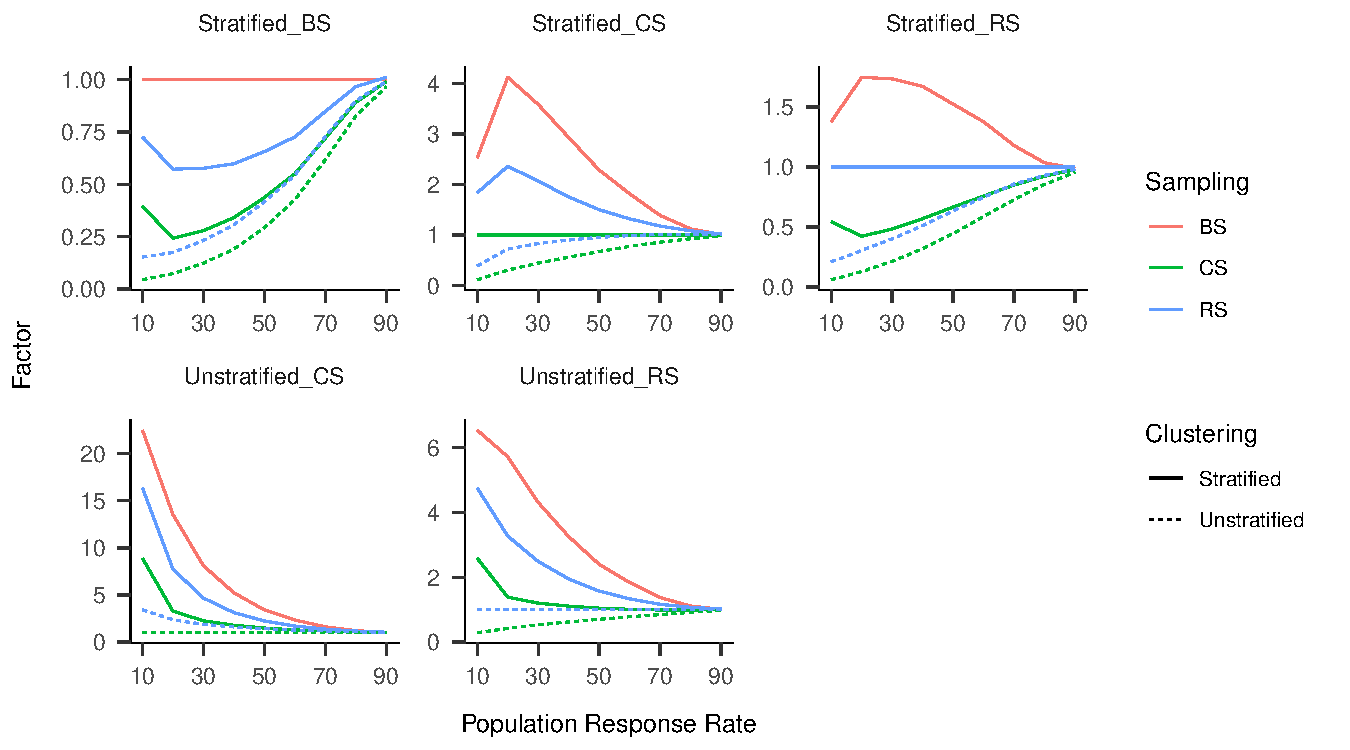
\includegraphics{GenSamp-Paper_files/figure-latex/fig-comp-1.pdf}
\caption{\label{fig:fig-comp}Relative sampling difficulty of each method compared to other methods. The straight horizontal line indicates the reference method being compared to.}
\end{figure}

\hypertarget{sampling-inequality-1}{%
\subsubsection{Sampling Inequality}\label{sampling-inequality-1}}

Figure \ref{fig:fig-gini-curve} displays the Gini curve and coefficient for all sampling methods across participation rates. The index is calculated by computing the area between the diagonal line and the curve. Coefficients of 0 indicate uniform equality across all sampling units, i.e.~all schools have an equal opportunity to be sampled. Coefficients of 1 indicate complete inequality, i.e.~very few schools are constantly being sampled across iterations. Overall, stratification results in lower inequality. However, since balanced sampling prioritizes schools according to set characteristics, the same schools are likely to be sampled each time.

\begin{sidewaysfigure}[p]
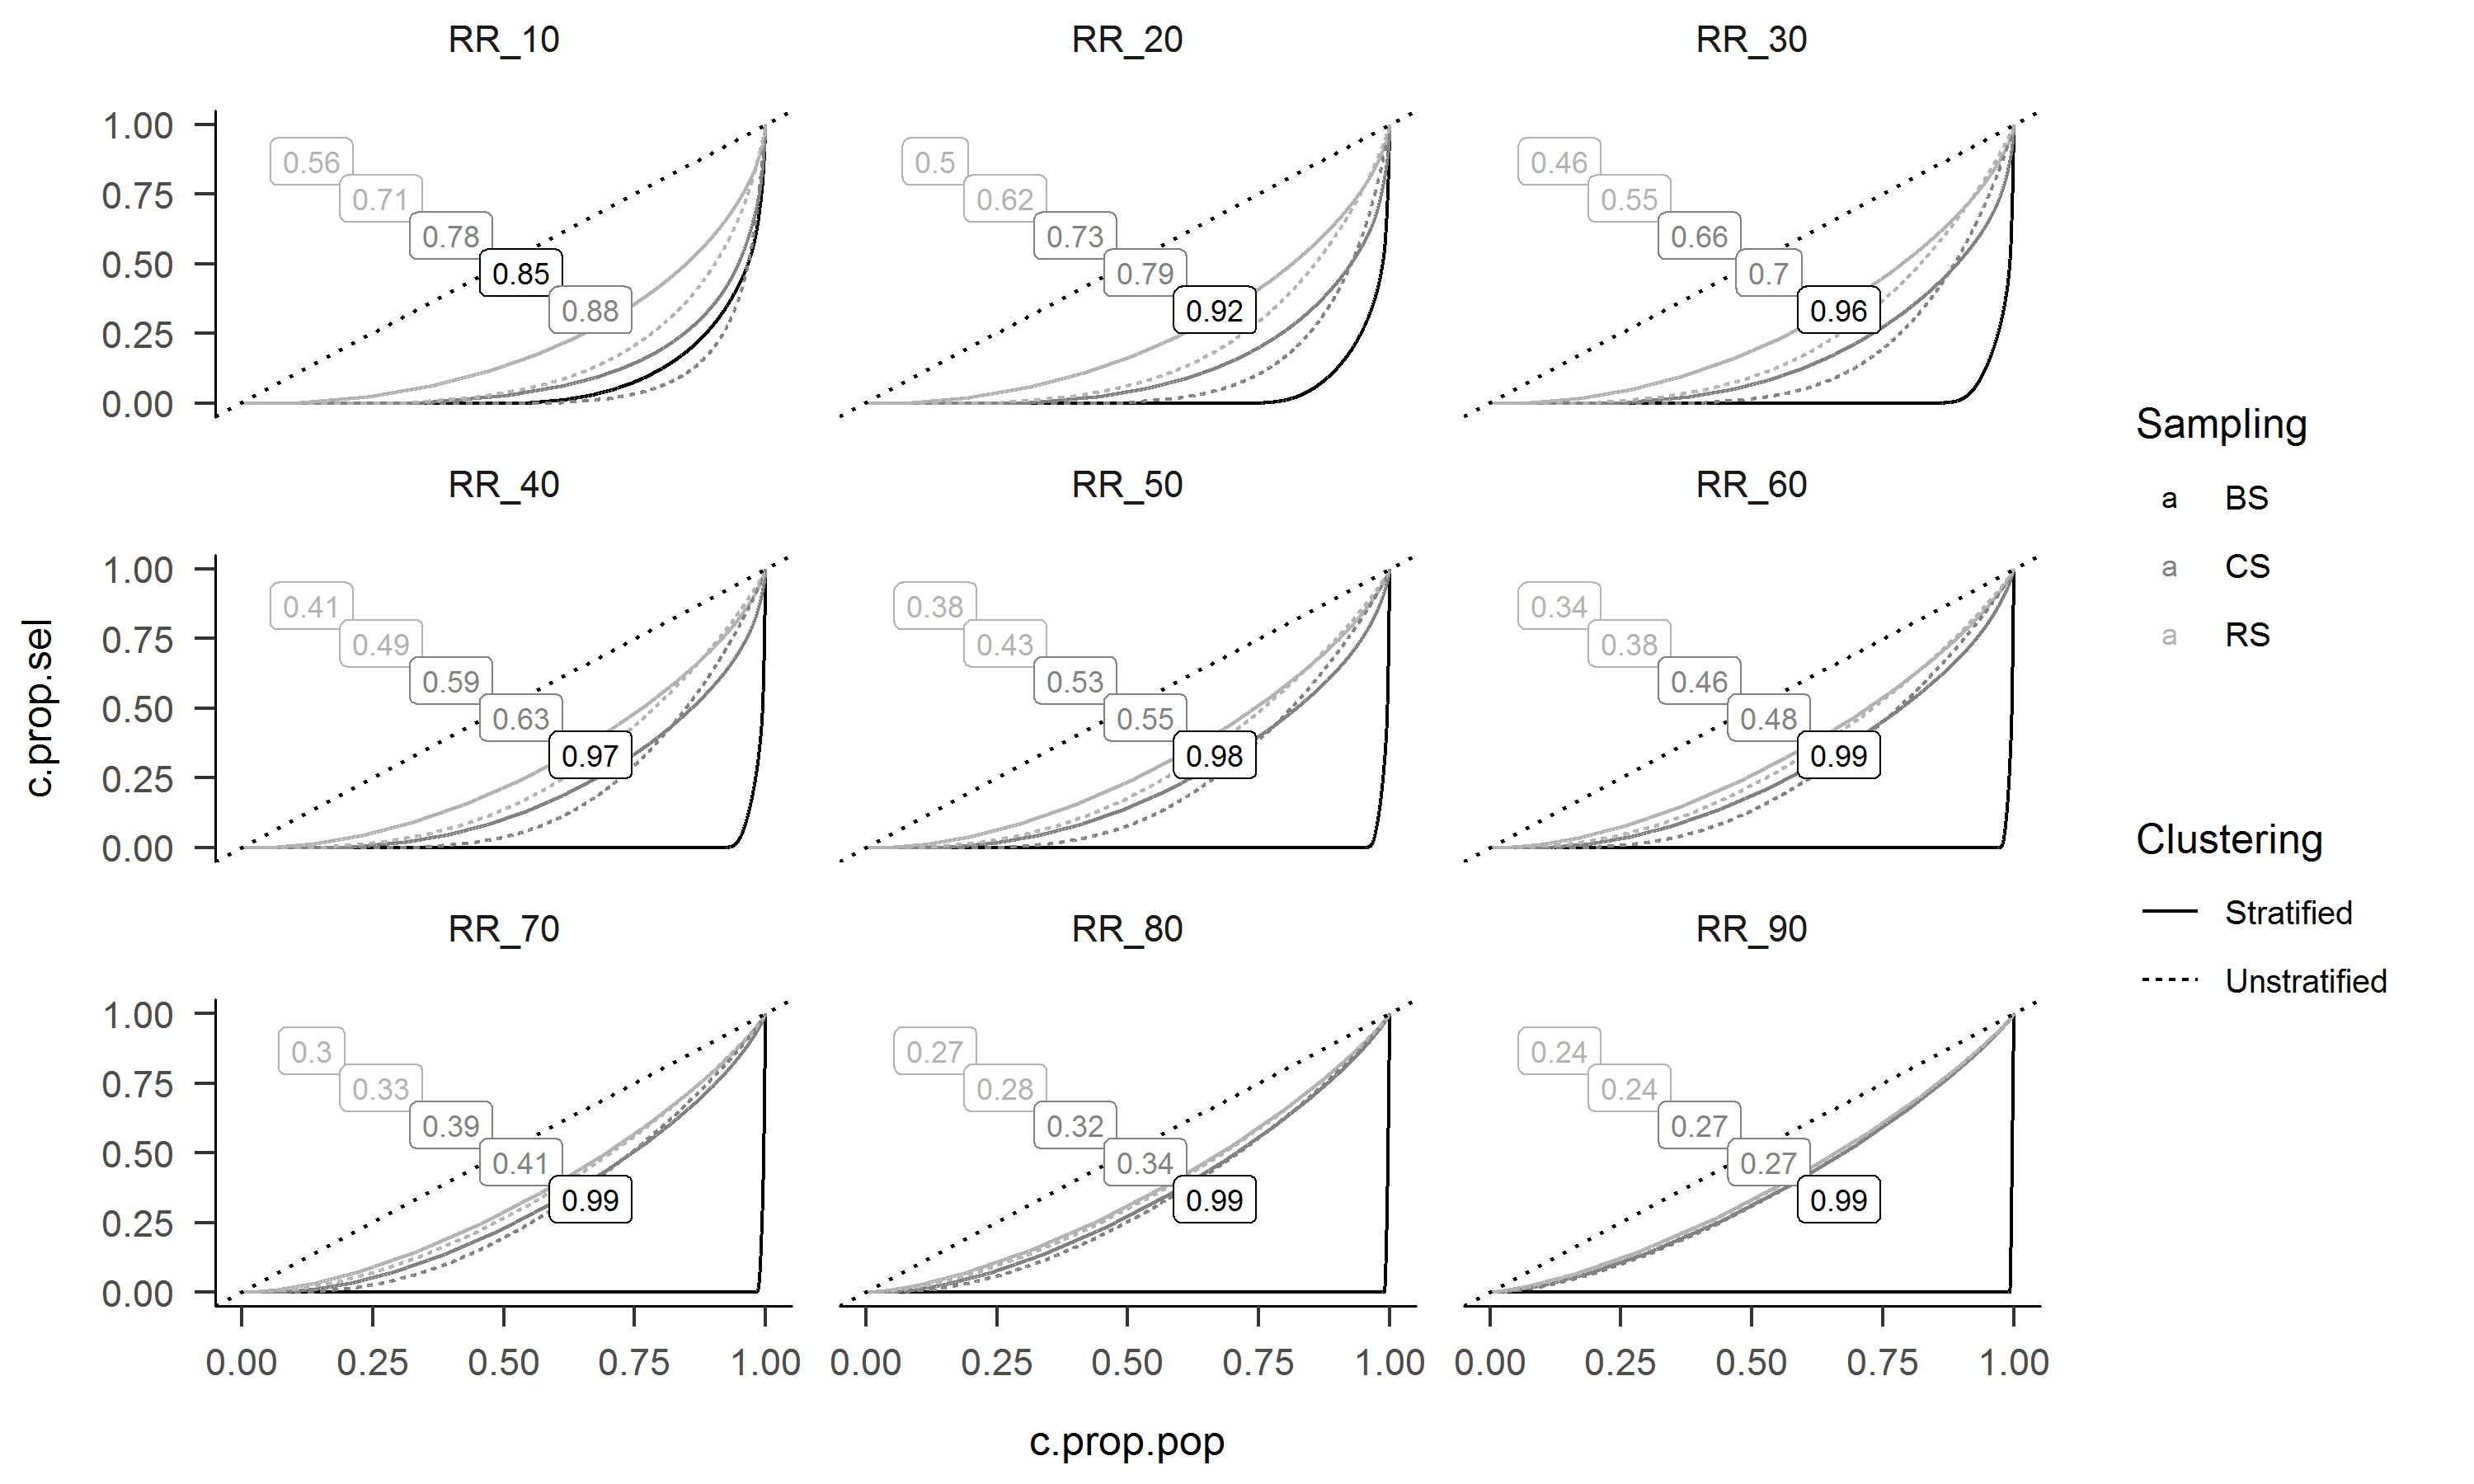
\includegraphics{GenSamp-Paper_files/figure-latex/fig-gini-curve-1} \caption{Cumulative probability plot and Gini coefficients representing the inequality of school sampling across sampling methods and population response rates.}\label{fig:fig-gini-curve}
\end{sidewaysfigure}

\newpage

\hypertarget{references}{%
\section{References}\label{references}}

\begingroup
\setlength{\parindent}{-0.5in}
\setlength{\leftskip}{0.5in}

\hypertarget{refs}{}
\leavevmode\hypertarget{ref-calinskiDendriteMethodCluster1974}{}%
Cali\a'nski, T., \& Harabasz, J. (1974). A dendrite method for cluster analysis. \emph{Communications in Statistics}, \emph{3}(1), 1--27. doi:\href{https://doi.org/10.1080/03610927408827101}{10.1080/03610927408827101}

\leavevmode\hypertarget{ref-fellersDevelopingApproachDetermine2017}{}%
Fellers, L. (2017). \emph{Developing an approach to determine generalizability: A review of efficacy and effectiveness trials funded by the Institute of Education Sciences} (Ph.D.). Columbia University, United States -- New York. Retrieved from \url{https://search.proquest.com/docview/1865595768/abstract/40FD82F4A0C24535PQ/1}

\leavevmode\hypertarget{ref-gerberFieldExperimentsDesign2012}{}%
Gerber, A. S., \& Green, D. P. (2012). \emph{Field experiments: Design, analysis, and interpretation} (1st ed.). New York: W. W. Norton.

\leavevmode\hypertarget{ref-gowerGeneralCoefficientSimilarity1971}{}%
Gower, J. C. (1971). A General Coefficient of Similarity and Some of Its Properties. \emph{Biometrics}, \emph{27}(4), 857--871. doi:\href{https://doi.org/10.2307/2528823}{10.2307/2528823}

\leavevmode\hypertarget{ref-grovesSurveyMethodology2004}{}%
Groves, R. M. (Ed.). (2004). \emph{Survey methodology}. Hoboken, N.J: Wiley-Interscience.

\leavevmode\hypertarget{ref-hennigHowFindAppropriate2013}{}%
Hennig, C., \& Liao, T. F. (2013). How to find an appropriate clustering for mixed-type variables with application to socio-economic stratification: How to Find an Appropriate Clustering. \emph{Journal of the Royal Statistical Society: Series C (Applied Statistics)}, \emph{62}(3), 309--369. doi:\href{https://doi.org/10.1111/j.1467-9876.2012.01066.x}{10.1111/j.1467-9876.2012.01066.x}

\leavevmode\hypertarget{ref-kernAssessingMethodsGeneralizing2016}{}%
Kern, H. L., Stuart, E. A., Hill, J., \& Green, D. P. (2016). Assessing Methods for Generalizing Experimental Impact Estimates to Target Populations. \emph{Journal of Research on Educational Effectiveness}, \emph{9}(1), 103--127. doi:\href{https://doi.org/10.1080/19345747.2015.1060282}{10.1080/19345747.2015.1060282}

\leavevmode\hypertarget{ref-olsenExternalValidityPolicy2013}{}%
Olsen, R. B., Orr, L. L., Bell, S. H., \& Stuart, E. A. (2013). External Validity in Policy Evaluations That Choose Sites Purposively. \emph{Journal of Policy Analysis and Management}, \emph{32}(1), 107--121. doi:\href{https://doi.org/10.1002/pam.21660}{10.1002/pam.21660}

\leavevmode\hypertarget{ref-omuircheartaighGeneralizingUnrepresentativeExperiments2014}{}%
O'Muircheartaigh, C., \& Hedges, L. V. (2014). Generalizing from unrepresentative experiments: A stratified propensity score approach. \emph{Journal of the Royal Statistical Society: Series C (Applied Statistics)}, \emph{63}(2), 195--210. doi:\href{https://doi.org/10.1111/rssc.12037}{10.1111/rssc.12037}

\leavevmode\hypertarget{ref-raudenbushStatisticalPowerOptimal2000}{}%
Raudenbush, S. W., \& Liu, X. (2000). Statistical power and optimal design for multisite randomized trials. \emph{Psychological Methods}, \emph{5}(2), 199--213. doi:\href{https://doi.org/10.1037//1082-989X.5.2.199}{10.1037//1082-989X.5.2.199}

\leavevmode\hypertarget{ref-shadishExperimentalQuasiexperimentalDesigns2002}{}%
Shadish, W. R., Cook, T. D., \& Campbell, D. T. (2002). \emph{Experimental and quasi-experimental designs for generalized causal inference}. Boston, MA, US: Houghton, Mifflin and Company.

\leavevmode\hypertarget{ref-steinleyKmeansClusteringHalfcentury2006}{}%
Steinley, D. (2006). K-means clustering: A half-century synthesis. \emph{British Journal of Mathematical and Statistical Psychology}, \emph{59}(1), 1--34. doi:\href{https://doi.org/10.1348/000711005X48266}{10.1348/000711005X48266}

\leavevmode\hypertarget{ref-stuartCharacteristicsSchoolDistricts2017}{}%
Stuart, E. A., Bell, S. H., Ebnesajjad, C., Olsen, R. B., \& Orr, L. L. (2017). Characteristics of School Districts That Participate in Rigorous National Educational Evaluations. \emph{Journal of Research on Educational Effectiveness}, \emph{10}(1), 168--206. doi:\href{https://doi.org/10.1080/19345747.2016.1205160}{10.1080/19345747.2016.1205160}

\leavevmode\hypertarget{ref-stuartUsePropensityScores2011}{}%
Stuart, E. A., Cole, S. R., Bradshaw, C. P., \& Leaf, P. J. (2011). The use of propensity scores to assess the generalizability of results from randomized trials: Use of Propensity Scores to Assess Generalizability. \emph{Journal of the Royal Statistical Society: Series A (Statistics in Society)}, \emph{174}(2), 369--386. doi:\href{https://doi.org/10.1111/j.1467-985X.2010.00673.x}{10.1111/j.1467-985X.2010.00673.x}

\leavevmode\hypertarget{ref-tiptonImprovingGeneralizationsExperiments2013}{}%
Tipton, E. (2013a). Improving Generalizations From Experiments Using Propensity Score Subclassification: Assumptions, Properties, and Contexts. \emph{Journal of Educational and Behavioral Statistics}, \emph{38}(3), 239--266. Retrieved from \url{https://www.jstor.org/stable/41999424}

\leavevmode\hypertarget{ref-tiptonStratifiedSamplingUsing2013}{}%
Tipton, E. (2013b). Stratified Sampling Using Cluster Analysis: A Sample Selection Strategy for Improved Generalizations From Experiments. \emph{Evaluation Review}, \emph{37}(2), 109--139. doi:\href{https://doi.org/10.1177/0193841X13516324}{10.1177/0193841X13516324}

\leavevmode\hypertarget{ref-tiptonHowGeneralizableYour2014}{}%
Tipton, E. (2014). How Generalizable Is Your Experiment? An Index for Comparing Experimental Samples and Populations. \emph{Journal of Educational and Behavioral Statistics}, \emph{39}(6), 478--501.

\leavevmode\hypertarget{ref-tiptonSiteSelectionExperiments2016}{}%
Tipton, E., Fellers, L., Caverly, S., Vaden-Kiernan, M., Borman, G., Sullivan, K., \& de Castilla, V. R. (2016). Site Selection in Experiments: An Assessment of Site Recruitment and Generalizability in Two Scale-up Studies. \emph{Journal of Research on Educational Effectiveness}, \emph{9}(sup1), 209--228. doi:\href{https://doi.org/10.1080/19345747.2015.1105895}{10.1080/19345747.2015.1105895}

\leavevmode\hypertarget{ref-tiptonImplicationsSmallSamples2017}{}%
Tipton, E., Hallberg, K., Hedges, L. V., \& Chan, W. (2017). Implications of Small Samples for Generalization: Adjustments and Rules of Thumb. \emph{Evaluation Review}, \emph{41}(5), 472--505. doi:\href{https://doi.org/10.1177/0193841X16655665}{10.1177/0193841X16655665}

\leavevmode\hypertarget{ref-tiptonImprovedGeneralizabilityImproved2019}{}%
Tipton, E., \& Matlen, B. J. (2019). Improved Generalizability Through Improved Recruitment: Lessons Learned From a Large-Scale Randomized Trial. \emph{American Journal of Evaluation}, \emph{40}(3), 414--430. doi:\href{https://doi.org/10.1177/1098214018810519}{10.1177/1098214018810519}

\endgroup


\end{document}
